
%----------------------------------------------------------------------------------------
%	PACKAGES AND OTHER DOCUMENT CONFIGURATIONS
%----------------------------------------------------------------------------------------

\documentclass[
11pt, % The default document font size, options: 10pt, 11pt, 12pt
%oneside, % Two side (alternating margins) for binding by default, uncomment to switch to one side
english, % ngerman for German
singlespacing, % Single line spacing, alternatives: onehalfspacing or doublespacing
%draft, % Uncomment to enable draft mode (no pictures, no links, overfull hboxes indicated)
%nolistspacing, % If the document is onehalfspacing or doublespacing, uncomment this to set spacing in lists to single
%liststotoc, % Uncomment to add the list of figures/tables/etc to the table of contents
%toctotoc, % Uncomment to add the main table of contents to the table of contents
%parskip, % Uncomment to add space between paragraphs
%nohyperref, % Uncomment to not load the hyperref package
headsepline, % Uncomment to get a line under the header
%chapterinoneline, % Uncomment to place the chapter title next to the number on one line
%consistentlayout, % Uncomment to change the layout of the declaration, abstract and acknowledgements pages to match the default layout
]{MastersDoctoralThesis} % The class file specifying the document structure

\usepackage[utf8]{inputenc} % Required for inputting international characters
\usepackage[T1]{fontenc} % Output font encoding for international characters

\usepackage{mathpazo} % Use the Palatino font by default

%\usepackage[backend=bibtex,style=authoryear]{biblatex} % Use the bibtex backend with the authoryear citation style (which resembles APA)
\usepackage[backend=bibtex,style=numeric,natbib=true]{biblatex} % Use the bibtex backend with numberic syle

% fixes issues with long url in citations
\usepackage{url}
\setcounter{biburllcpenalty}{7000}
\setcounter{biburlucpenalty}{8000}


\addbibresource{thesis.bib} % The filename of the bibliography

\usepackage[autostyle=true]{csquotes} % Required to generate language-dependent quotes in the bibliography


%----------------------------------------------------------------------------------------
%	MARGIN SETTINGS
%----------------------------------------------------------------------------------------

\geometry{
	paper=a4paper, % Change to letterpaper for US letter
	inner=2.5cm, % Inner margin
	outer=3.8cm, % Outer margin
	bindingoffset=.5cm, % Binding offset
	top=1.5cm, % Top margin
	bottom=1.5cm, % Bottom margin
	%showframe, % Uncomment to show how the type block is set on the page
}

%----------------------------------------------------------------------------------------
%	CUSTOM CHANGES
%----------------------------------------------------------------------------------------

% packages
\usepackage{hyperref}
\usepackage{amsmath}
\usepackage{enumitem}
\usepackage{graphicx}
\usepackage[all]{hypcap}
\usepackage{caption}
\usepackage{subcaption}

% new commands
\newcommand{\B}[1]{\textbf{#1}}
\newcommand{\I}[1]{\textit{#1}}
\newcommand{\U}[1]{\underline{#1}}


%----------------------------------------------------------------------------------------
%	THESIS INFORMATION
%----------------------------------------------------------------------------------------

\thesistitle{Thesis Title} % Your thesis title, this is used in the title and abstract, print it elsewhere with \ttitle	
\supervisor{Prof. Gabriel Wittum} % Your supervisor's name, this is used in the title page, print it elsewhere with \supname
\examiner{} % Your examiner's name, this is not currently used anywhere in the template, print it elsewhere with \examname
\degree{Bachelor of Science} % Your degree name, this is used in the title page and abstract, print it elsewhere with \degreename
\author{Marvin Glaser} % Your name, this is used in the title page and abstract, print it elsewhere with \authorname
\addresses{} % Your address, this is not currently used anywhere in the template, print it elsewhere with \addressname

\subject{Computer Science} % Your subject area, this is not currently used anywhere in the template, print it elsewhere with \subjectname
\keywords{} % Keywords for your thesis, this is not currently used anywhere in the template, print it elsewhere with \keywordnames
\university{\href{https://www.goethe-university-frankfurt.de/}{Goethe-University Frankfurt}} % Your university's name and URL, this is used in the title page and abstract, print it elsewhere with \univname
\department{\href{https://gcsc.uni-frankfurt.de/}{Goethe Center for Scientific Computing (G-CSC)}} % Your department's name and URL, this is used in the title page and abstract, print it elsewhere with \deptname
\group{\href{}{Epidemics Group}} % Your research group's name and URL, this is used in the title page, print it elsewhere with \groupname
\faculty{\href{http://faculty.university.com}{Faculty Name}} % Your faculty's name and URL, this is used in the title page and abstract, print it elsewhere with \facname

\AtBeginDocument{
\hypersetup{pdftitle=\ttitle} % Set the PDF's title to your title
\hypersetup{pdfauthor=\authorname} % Set the PDF's author to your name
\hypersetup{pdfkeywords=\keywordnames} % Set the PDF's keywords to your keywords
}

\begin{document}

\frontmatter % Use roman page numbering style (i, ii, iii, iv...) for the pre-content pages

\pagestyle{plain} % Default to the plain heading style until the thesis style is called for the body content




%----------------------------------------------------------------------------------------
%	TITLE PAGE
%----------------------------------------------------------------------------------------

\begin{titlepage}
\begin{center}

\vspace*{.06\textheight}
{\scshape\LARGE \univname\par}\vspace{1.5cm} % University name
\textsc{\Large Bachelor Thesis}\\[0.5cm] % Thesis type

\HRule \\[0.4cm] % Horizontal line
{\huge \bfseries \ttitle\par}\vspace{0.4cm} % Thesis title
\HRule \\[1.5cm] % Horizontal line
 
\begin{minipage}[t]{0.4\textwidth}
\begin{flushleft} \large
\emph{Author:}\\
\href{http://www.johnsmith.com}{\authorname} % Author name - remove the \href bracket to remove the link
\end{flushleft}
\end{minipage}
\begin{minipage}[t]{0.4\textwidth}
\begin{flushright} \large
\emph{Supervisor:} \\
\href{http://www.jamessmith.com}{\supname} % Supervisor name - remove the \href bracket to remove the link  
\end{flushright}
\end{minipage}\\[3cm]
 
\vfill

\large \textit{A thesis submitted in fulfillment of the requirements\\ for the degree of \degreename}\\[0.3cm] % University requirement text
\textit{in the}\\[0.4cm]
\groupname\\\deptname\\[2cm] % Research group name and department name
 
\vfill

{\large \today}\\[4cm] % Date
%\includegraphics{Logo} % University/department logo - uncomment to place it
 
\vfill
\end{center}
\end{titlepage}

%----------------------------------------------------------------------------------------
%	DECLARATION PAGE
%----------------------------------------------------------------------------------------

\begin{declaration}
\addchaptertocentry{\authorshipname} % Add the declaration to the table of contents
\noindent I, \authorname, declare that this thesis titled, \enquote{\ttitle} and the work presented in it are my own. I confirm that:
\label{declaration}
\begin{itemize} 
\item This work was done wholly or mainly while in candidature for a research degree at this University.
\item Where any part of this thesis has previously been submitted for a degree or any other qualification at this University or any other institution, this has been clearly stated.
\item Where I have consulted the published work of others, this is always clearly attributed.
\item Where I have quoted from the work of others, the source is always given. With the exception of such quotations, this thesis is entirely my own work.
\item I have acknowledged all main sources of help.
\item Where the thesis is based on work done by myself jointly with others, I have made clear exactly what was done by others and what I have contributed myself.\\
\end{itemize}
 
\noindent Signed:\\
\rule[0.5em]{25em}{0.5pt} % This prints a line for the signature
 
\noindent Date:\\
\rule[0.5em]{25em}{0.5pt} % This prints a line to write the date
\end{declaration}

\cleardoublepage

%----------------------------------------------------------------------------------------
%	QUOTATION PAGE
%----------------------------------------------------------------------------------------

%\vspace*{0.2\textheight}
%
%\noindent\enquote{\itshape Thanks to my solid academic training, today I can write hundreds of words on
%virtually any topic without possessing a shred of information, which is how I got a good job in journalism.}\bigbreak
%
%\hfill Dave Barry

%----------------------------------------------------------------------------------------
%	ABSTRACT PAGE
%----------------------------------------------------------------------------------------

%\begin{abstract}
%\addchaptertocentry{\abstractname} % Add the abstract to the table of contents
%The Thesis Abstract is written here (and usually kept to just this page). The page is kept centered vertically so can expand into the blank space above the title too\ldots
%\end{abstract}

%----------------------------------------------------------------------------------------
%	LIST OF CONTENTS/FIGURES/TABLES PAGES
%----------------------------------------------------------------------------------------

\tableofcontents % Prints the main table of contents

%\listoffigures % Prints the list of figures

%\listoftables % Prints the list of tables

%----------------------------------------------------------------------------------------
%	ABBREVIATIONS
%----------------------------------------------------------------------------------------

%\begin{abbreviations}{ll} % Include a list of abbreviations (a table of two columns)
%
%\textbf{LAH} & \textbf{L}ist \textbf{A}bbreviations \textbf{H}ere\\
%\textbf{WSF} & \textbf{W}hat (it) \textbf{S}tands \textbf{F}or\\
%
%\end{abbreviations}

%----------------------------------------------------------------------------------------
%	PHYSICAL CONSTANTS/OTHER DEFINITIONS
%----------------------------------------------------------------------------------------

%\begin{constants}{lr@{${}={}$}l} % The list of physical constants is a three column table
%
%% The \SI{}{} command is provided by the siunitx package, see its documentation for instructions on how to use it
%
%%Speed of Light & $c_{0}$ & \SI{2.99792458e8}{\meter\per\second} (exact)\\
%%Constant Name & $Symbol$ & $Constant Value$ with units\\
%
%\end{constants}

%----------------------------------------------------------------------------------------
%	DEDICATION
%----------------------------------------------------------------------------------------

%\dedicatory{For/Dedicated to/To my\ldots} 

%----------------------------------------------------------------------------------------
%	THESIS CONTENT - CHAPTERS
%----------------------------------------------------------------------------------------

\mainmatter % Begin numeric (1,2,3...) page numbering

\pagestyle{thesis} % Return the page headers back to the "thesis" style

% Include the chapters of the thesis as separate files from the Chapters folder
% Uncomment the lines as you write the chapters

% Chapter Template

\chapter{Introduction and Motivation} % Main chapter title

\label{chap:introduction} % Change X to a consecutive number; for referencing this chapter elsewhere, use \ref{ChapterX}

%----------------------------------------------------------------------------------------
%	SECTION 1
%----------------------------------------------------------------------------------------
\section{Motivation}
Throughout human history, humanity has struggled with overcoming the outbreak of diseases.
Bacteria, viruses, parasites and other causes for sickness are omnipresent on our planet\cite{balloux2017q}. Some are
relatively easy to overcome for most individuals, like Influenza\cite{cdc_influenza}. Others, like the human immunodeficiency viruses (HIV),
can have a severe impact on an individual's life\cite{chaponda2018systematic,ji2007impact}. In addition to the impact sickness has
on the live of individuals, diseases and how they spread, have a huge impact on our societies. Hospitals need to be 
build and staffed with doctors, nurses and other facility members. Supply chains need to be established and maintained in order
to manufacture drugs and materials that can be used to cure patients. Research must be conducted, and new treatments need to be
established to increase the chances of a positive outcome. This entire network of services is costly in terms of time, effort
and money used to both establish and maintain it. It is therefor incredibly important to control the spread of diseases early,
in order to prevent damages on both an individual and an economical level.
A good example for the impacts of a rapidly spreading disease is the ongoing ``severe acute respiratory syndrome coronavirus 2''
(SARS-CoV-2 or COVID-19) pandemic. Much political and scientific debate in the past two years has revolved around options to better
understand and predict the properties that cause the rapid spreading of this disease. 

%In 2019, the United States of America spend
%16.77\% of their GDP (gross domestic product) on healthcare expenditures\cite{WHO site}. This shows that managing public health
%is important for every society in order to both stay competitive economically and provide citizens with a high quality of live.\newline
%----------------------------------------------------------------------------------------
%	SECTION 2
%----------------------------------------------------------------------------------------
\section{Research goals}
This work aims to contribute to the previously mentioned field
and build on the work of Rastogi et al.\cite{Rastogi}. In his work the ``SEIRD'' model\cite{Wittum1,Wittum2} was used to
model the spreading of COVID-19 in 7 major cities of Germany on a 2-dimensional grid (2-D grid). This work follows up on this, by
modeling COVID-19 spreading in the 26 interconnected region of Hesse, Germany. In doing so we focus on the following questions.

\begin{enumerate}
	\item How well does the SEIRD model performs in a setting with more regions?
	\item How well does the current optimization strategy work?
	\item What are potential areas of improvement of the model?
\end{enumerate}

In order to achieve these goals the SEIRD model was modified in an effort to better represent the conditions of the real world.
Additionally modifications to the model implementation were introduced to enable the model to clearly differentiate between different
regions on the grid. Lastly the model was tested with different data conditions, and the results analyzed in multiple ways.
%\par
%Even though huge progress has been made in the fight against infectious diseases (a notable example being the eradication of
%small pox\cite{??}), sickness due to infectious diseases remain a common phenomenon in modern civilizations. Viruses are
%among the most successful organisms in spreading between populations of both humans and animals\cite{??}. The most notable example
%for this is the currently ongoing ``severe acute respiratory syndrome coronavirus 2'' (SARS-CoV-2) pandemic. The SARS-CoV-2 or
%coronavirus disease 2019 (short COVID-19) was first observed in an outbreak in the Chinese city of Wuhan in December 2019\cite{??}.
%From there it started to spread around the globe and on March, 11 2020, the world health organization declared a world wide pandemic\cite{??}.\newline
%\par
%Managing this pandemic has been a huge challenge in the past two years and much debate has revolved around managing the spread of this
%infectious disease. To this end, scientists from many different fields have researched the properties of this virus in order to better
%understand and predict how COVID-19 spreads in our societies. One of these fields is a branch of computer science and math, that aims to
%model the spread of infectious diseases, such as  COVID-19, using differential equations. This work aims to contribute to this field and
%%provide insight in the process of modeling the spread of infectious diseases on a two-dimensional grid using the SEIRD method. 
%provide insight in the process of modeling the spread of infectious diseases, by building on the work of Rastogi et al.\cite{rastogi}.
%In this work the ``SEIRD'' model\cite{wittum} was applied to seven major cities of Germany on a 2-dimensional (2D) grid. This work
%follows up on this, by simulating COVID-19 spreading on 26 interconnected regions in the federal state of Hesse, Germany.



%\section{Aims and goals}
%\textcolor{red}{Maybe move this more to the beginning? Difficult to formulate without previous explanations...}\newline % note
%\textcolor{red}{difficult to explain without model introduction}\newline % note
%This work aims to provide insight into the nature of the spreading of the COVID-19 virus. In a previous work Rastogi et al.\cite{rastogi}
%\textcolor{red}{(check for correct BA citation style)} % note
%explored the capability of the ``SEIRD'' model\cite{wittum} (detailed explanation in the \hyperref[sec:SEIRD]{following sections}).
%In his work he simulated the features of the COVID-19 pandemic in seven major cities of Germany on a 2-dimensional (2D) grid. While the
%results are interesting it remained unclear, how the model performs when simulating interconnected areas in a larger landscape.\newline
%
%\par
%In order to better understand the SEIRD model, a 2D grid of the German region of Hesse was created and used to simulate the spreading of
%the COVID-19 virus in the uninfected portion of the population. In addition, two parameters, that are regulating the spreading behavior
%in the model, were investigated closer. This analysis aimed to better understand the influence of the individual parameters on the modeling
%process itself.


% Chapter Template

\chapter{Theory} % Main chapter title
This chapter focuses on explaining the general theory behind the model and the methods used in this work.
Details regarding the exact problem definition, model adjustments, programs used and so on are given in
\hyperref[chap:methods]{Chapter \ref*{chap:methods}}.


\label{chap:theory} % Change X to a consecutive number; for referencing this chapter elsewhere, use \ref{ChapterX}

%----------------------------------------------------------------------------------------
%	SECTION 1
%----------------------------------------------------------------------------------------

\section{Compartmental modeling techniques}
Compartmental modeling revere to a modeling technique often used to systematically describe real world phenomena
like disease spreading\cite{compartementMod}. In these models the population is divided into different groups. 
Members of one group can move to another group. This movement is based on equations that are used to model the real
world behavior of each group. The following two sections introduce both the ``SIR'' and the ``SEIRD'' model. The
latter model was the focus on this work.

%-----------------------------------
%	SUBSECTION 1
%-----------------------------------
\subsection{Ordinary differential equations}

%-----------------------------------
%	SUBSECTION 2
%-----------------------------------
\subsection{Partial differential equations}


%-----------------------------------
%	SUBSECTION 3
%-----------------------------------
\subsection{The SIR model}
\label{sec:SIR}
In 1927 \cite{kermack1991contributions} first introduced their method to mathematically describe  
the course  of an infectious disease. The model divides a population into three distinct groups.

\begin{enumerate}[label=$\bullet$]
	\item \B{Susceptibles (S)}: Individuals that are naive to the infection and hence not immune. If in contact with
		the virus these individuals can migrate to the\linebreak ``Infected'' group
	\item \B{Infected (I)}: Individuals that are infected with the disease. Infected individuals contribute to the 
		infection of members of the susceptible group. At some point during their infection, these members
		transition to the ``Removed'' group.
	\item \B{Removed (R)}: Individuals that  have either overcome their infection and are now immune to the disease
		or have succumb to the disease and are diseased. They do not spread the virus and cannot be infected again.
\end{enumerate}

\par
The population changes of all three groups are described by mathematical equations\cite{mathSIR}. Notable variables
are the number of susceptible members (S), number of infected members (I), number of recovered members (R), $\alpha$
which is a positive constant that describes the transmission rate of the disease and $\beta$, which is a positive
constant between 0 and 1 that describes the transition rate (either recovery or death) between \B{I} and \B{R}.
$\beta$ can be rewritten as $\frac{1}{b}$, where $b$ is the average duration an infected individual remains infectious,
before it either recovers or dies. The model is illustrated in \hyperref[fig:SIR]{Figure \ref*{fig:SIR}}, the equations
are expressed as follows:

\begin{figure}
	\begin{center}
		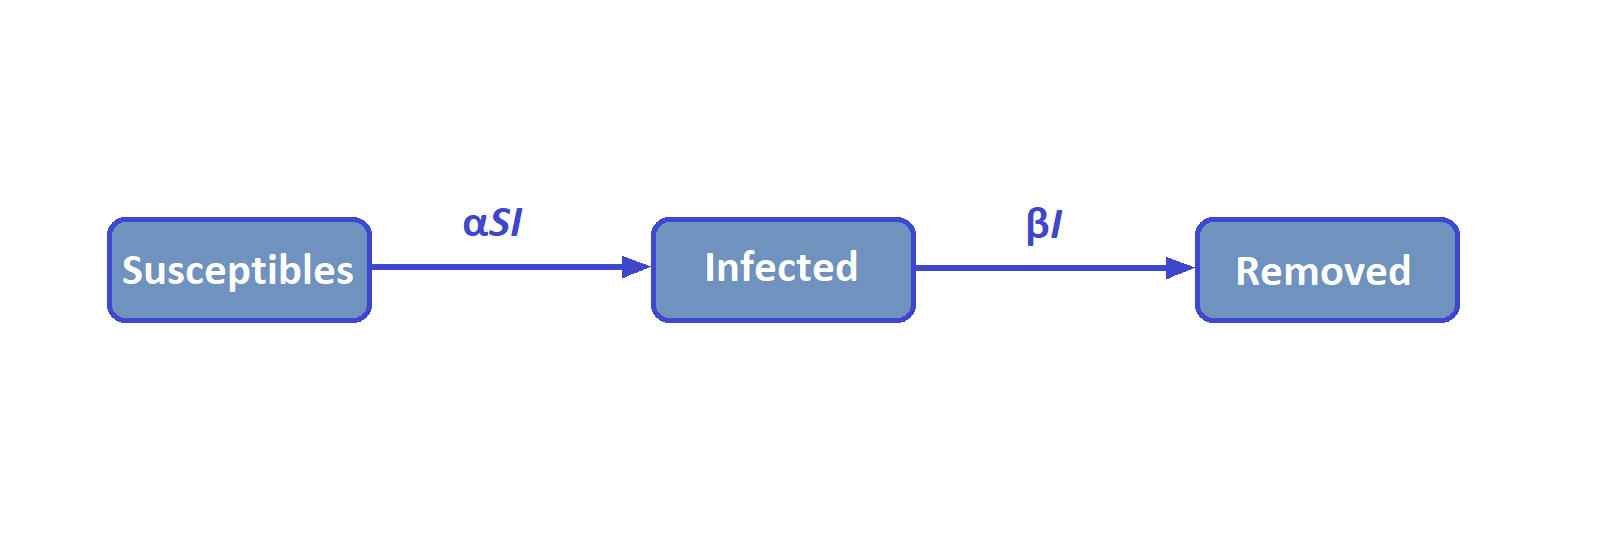
\includegraphics[width=0.75\textwidth]{./figures/SIR.png}
		\caption{Illustration of the population flow in the SIR model. S represents the ``Susceptible'', I
			the ``Infected'' and R the ``Removed'' population. The variable $\beta$ can also redefined
			as $\frac{1}{b}$, where $D$ is the average duration of infectiousness}
		\label{fig:SIR}
	\end{center}
\end{figure}


\begin{align}
	\label{eq:SIR1}
	\frac{dS}{dt} &= -\alpha S I \\
	\frac{dI}{dt} &= \alpha S I - \beta I \\
	\frac{dR}{dt} &= \beta I
\end{align}

\par
The model also assumes the total number of individuals in the system $N$ remains constant and that the sum of all transitions
between all three groups during every time step remains zero. This is expressed in the equations below.
$S(t)$, $I(t)$ and $R(t)$ express the number of individuals in each of the groups, at time $t$, respectively.

\begin{align}
	\label{eq:SIR2}
	I(t) + S(t) + R(t) &= N \\
	\frac{dS}{dt} + \frac{dI}{dt} + \frac{dR}{dt} = 0
\end{align}

\par
Since the model assumes, that the total population remains stable, phenomena like immigration or child birth are not accounted
for. This does not correctly represent the real world. However it is often assumed, that population fluctuations
due to these occurrences are minor enough compared to the entirety of a regions population, that they do not alter the results of the
simulation in a major way\cite{??}.\newline

\par
In order to correctly model the dynamics of an epidemic, the variables of these differential
equations (like $\alpha$ and $\beta$ in this case) must be determined correctly. This process is referred to as solving the equations.
Different techniques exist to do so. Two of these techniques are the \hyperref[sec:Gauss]{Gauss-Newton algorithm}\cite{Gauss??} and
\hyperref[sec:PSO]{Particle Swarm Optimization (PSO)}\cite{PSO??}. Both of these techniques will are explained in a later section.


%-----------------------------------
%	SUBSECTION 4
%-----------------------------------

\subsection{The SEIRD model}
\label{sec:SEIRD}
The SEIRD model is a variant of the simpler SIR model\cite{knodel20173d}
\textcolor{red}{(double check citation)}. % note
It introduces two new groups and describes the status for the infected population much more precise. The groups of the SEIRD
model are as follows:

\begin{enumerate}[label=$\bullet$]
	\item \B{Susceptibles (S)}: Individuals that are naive to the infection and hence not immune (identical to SIR).
	\item \B{Exposed (E)}: Individuals that are infected, but show no or very little symptoms. These individuals
		do not quarantine (yet) and are therefor contributing to the spread of the virus.
	\item \B{Infected (I)}: Individuals that have developed such a sever illness, that they need to be hospitalized.
	\item \B{Recovered (R)}: Individuals that  have overcome the infection and are now immune to the disease.
	\item \B{Diseased (D)}: Individuals that have succumb to the infection.
\end{enumerate}

\par
As described in the previous section, transition between the Individuals of different groups is a core
part of the model. The transition between the \B{S} and \B{E} population in SEIRD is equivalent to the transition
between \B{S} and \B{I} in SIR. However, the population outflow from the \B{E} group is split and can either move
to the \B{I} or to the \B{R} group. This allows the modeling of infections that result in quick recovery or an infection
with complications (defined by the hospitalization of the patient). The ratio between the two scenarios is governed by the variable
$\kappa$. In addition, the variable $q$ was introduced and now represents the average duration until recovery/hospitalization of an
infected individual. Similarly, the outflow of \B{I} is split between the populations of \B{R} and \B{D}. The ratio is governed
by the variable $\tau$. The equations for \B{R} and \B{D} were also adjusted to represent these changes. Lastly $D$ was redefined
as $p$, which now represents the average of a hospitalized individual to either recover or succumb to the infection.
\hyperref[fig:SEIRD]{Figure \ref*{fig:SEIRD}} illustrates all these changes. The modified equations are as follows:

\begin{align}
	\label{eq:SEIRD1}
	\frac{dS}{dt} &= -\alpha S E \\
	\frac{dE}{dt} &= \alpha S E -\frac{1}{q} E \\
	\frac{dI}{dt} &= \frac{\kappa}{q} E - \frac{1}{p} I \\
	\frac{dR}{dt} &= \frac{1-\kappa}{q} E + \frac{1-\tau}{p} I \\
	\frac{dD}{dt} &= \frac{\tau}{p} I
\end{align}


\begin{figure}
	\begin{center}
		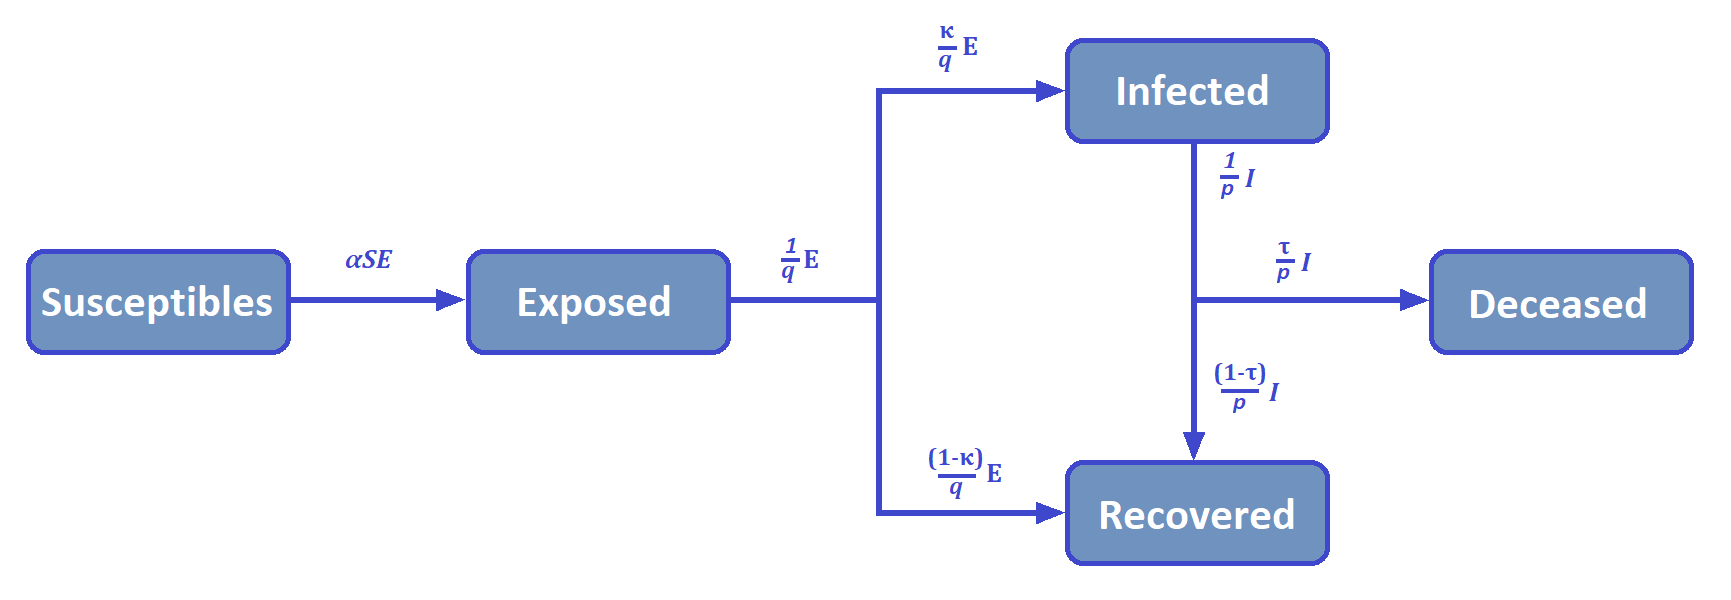
\includegraphics[width=0.75\textwidth]{./figures/SEIRD.png}
		\caption{Illustration of the population flow in the SEIRD model. S represents the ``Susceptible'', E the ``Exposed'',
			I the ``Infected'', R the ``Recovered'' and D the ``Diseased'' population. $\beta$ can also be expressed as
			$\frac{1}{\phi}$, where $\phi$ is the average time to recovery/hospitalization.}
		\label{fig:SEIRD}
	\end{center}
\end{figure}


\par
Like SIR, the SEIRD model assumes that the total number of individuals $N$ in the population remains constant during every step
of the modeling process. This leads to the equations expressed below. Again, $S(t)$, $E(t)$, $I(t)$, $R(t)$ and $D(t)$ are
expressing the number of individuals for each group at time $t$, respectively. $N$ remains the total number of individuals in the model.

\begin{align}
	\label{eq:SEIRD2}
	S(t) + E(t) + I(t) + R(t) + D(t) &= N \\
	\frac{dS}{dt} + \frac{dE}{dt}  + \frac{dI}{dt} + \frac{dR}{dt} + \frac{dD}{dt} = 0
\end{align}

\par
A model like this expresses the dynamics of an epidemic in much more detail. A weakness of the SIR model is that it does distinct between important
groups such as sick, but not infected and hospitalized individuals. The SEIRD model is capable of doing so and also allows for predicting
figures like the number of hospitalized individuals at time $t$.\newline

\par
This work focused mostly on the modeling capability of SIR in the transition stage between susceptibles and exposed. To better fulfill this
task, the model was redefined to accommodate for a lack of clear source data and to further refine the modeling of real wold phenomena. The changes
are described in detail in \hyperref[sec:SEIRDredef]{chapter~\ref*{chap:methods}, section~\ref*{sec:SEIRDredef}}.



%----------------------------------------------------------------------------------------
%	SECTION 2
%----------------------------------------------------------------------------------------

\section{Variable optimization algorithms}
In order for the presented models to work properly, it is important to determine the correct value for each unknown variable. There are many
methods to determine these variables. In the context of differential equations this process is often referred to as ``solving'' the equations.
Algorithms and methods that try to achieve this are generally referred to as ``solvers''.\newline

\par
The following sections will explain two methods used in this work. The Gauss-Newton algorithm and the Particle Swarm Optimization algorithm (PSO).

%-----------------------------------
%	SUBSECTION 1
%-----------------------------------

\subsection{Gauss-Newton algorithm}
\label{sec:Gauss}

%-----------------------------------
%	SUBSECTION 2
%-----------------------------------

\subsection{Particle Swarm Optimization}
\label{sec:PSO}

% Chapter Template

\chapter{Methodology} % Main chapter title
The following chapter will describe the problem that investigated in this work, the model adjustments and definitions,
the methods and the tools used to do so.

\label{chap:methodology} % Change X to a consecutive number; for referencing this chapter elsewhere, use \ref{ChapterX}

%----------------------------------------------------------------------------------------
%	SECTION 1
%----------------------------------------------------------------------------------------

\section{Problem definition}
\label{sec:problemDef}
%The goal of modeling is always to invent a model that is capable of correctly reproducing past and reliably predicting 
%future events. The latter is often very difficult, since it is necessary to correctly understand the dynamics of a
%complex system and then implement these dynamics in the form of a program, algorithm or method.\newline

%\par
The previous work of \cite{Rastogi} investigated the SEIRD model on a 2d-grid of Germany. In his work he simulated
all five groups of the SEIRD model for seven cities in Germany. This proved that the model itself is functional and
in principle capable of reproducing and predicting the dynamic of the COVID-19 pandemic or other pandemic/endemic events. \newline

\par
The goal of this work was to better understand the performance of the model in a smaller scale environment and to improve
the quality of the results. Hesse (Germany) and its regions where chosen as a template for a new 2d-grid. To minimize the
propagation of error throughout the SEIRD groups, we decided to focus on optimizing the fist class individuals, the Susceptible (\B{S}) group.
In this context we tried to reproduce/predict real world data and upcoming trends. Additionally we focused on evaluating the
sensitivity of \B{S} to the two variables $\alpha$ and $q$.

%-----------------------------------
%	SECTION 2
%-----------------------------------
\section{Data acquisition and model adjustment}
The following section will explain the processes of data acquisition, issues and modifications of the SEIRD model,
in order to improve the quality of the results.

%-----------------------------------
%	SUBSECTION 1
%-----------------------------------
\subsection{Data acquisition}
\label{sec:datacoll}
In order to perform SEIRD simulations, it was necessary to gather precise real world data for as many of the five groups as possible.
The source for this data was the Github project \cite{Gehrcke}, which provided both the number of COVID-19 infections,
as well as the number of COVID-19 related deaths per region in Germany. The repository provides data based on the case/death
numbers published by the RKI (Robert Koch Institute) and the Risklayer GmbH. In this work the data based on the RKI publications
was used. The data format were cumulative case/death numbers per region per day.\newline

\par
The hospitalization rate of confirmed COVID-19 infected individuals, the average time till symptom onset, the average time till
hospitalization and the lethality rate case of an infection was taken from RKI publications \cite{RKIcov}. At the time of acquisition, these
numbers were only estimations based on the literature of the current date.\newline

\par
The population of each region in Hesse was taken from the website ``statistic.hessen.de''. The data was sourced from \cite{HessePop}
in the category ``Bef\"olkerung in Hessen 2017 bis 2020 nach Verwaltungsbezirk in Monaten''. The size of each region in Hesse
was taken from \cite{HesseSize}.

%-----------------------------------
%	SUBSECTION 2
%-----------------------------------
\subsection{SEIRD model adjustments}
\label{sec:SEIRDredef}
In order to reach the goals described in \hyperref[sec:problemDef]{section \ref*{sec:problemDef}}, we decided to alter
the definitions of the Exposed (\B{E}) and Infected (\B{I}) groups. Furthermore we decided to set the variable
$\kappa$ to 1, effectively removing the option of exposed individuals to recover without developing symptoms. These
changes were done for two major reasons:\newline

\par
First, data availability proved to be an issue. The problem being, that the number of infected in the
collected data set only includes individuals where the COVID-19 pathogen could be isolated or that were tested positive
with a polymerase chain reaction (PCR) or antigen test\cite{RKIcase}. However,
these tests are usually conducted, if an individual is experiencing symptoms of sickness. This means, that individuals, that do
not experience symptoms were (for the most part) not represented in the collected data. In addition, it was difficult to estimate
the ratio between infected individuals that experience symptoms and individuals that do not experience symptoms. This made it
even harder make realistic assumptions, on which bases the original data could be modified to account for this phenomenon.\newline

\par
The second reason for these changes is a better representation of the actual disease history of COVID-19. Many infections
between susceptible and exposed individuals happen, before the exposed develop symptoms. While sick individuals can infect others many
days after symptom onset, about halve of all transmissions are pre-symptomatic \cite{casey2021presymptomatic} and that symptom onset generally
reduces transmission rates due to isolation measures\cite{RKIcov}.

\par
Based on this information, we did not allow for direct recovery from the model and redefined redefined the \B{E} and \B{I} groups as follows.
\begin{enumerate}[label=$\bullet$]
	\item \B{Exposed (E)}: Group of individuals that are infected with the virus and will develop symptoms in the upcoming
		days. Individuals are contagious during this time and contribute to infections of susceptibles.
	\item \B{Infected (I)}: Group of individuals that has experienced symptoms. Individuals are mostly not contagious anymore
		and isolate themself/are isolated until recovery or death.
\end{enumerate}

Of course these assumptions are not fully representative of the real world dynamics of COVID-19 disease spreading. However, based on
the information described prior, we think that these changes improve the overall accuracy of the model and the interpretation of real world data.

%----------------------------------------------------------------------------------------
%	SECTION 2
%----------------------------------------------------------------------------------------

\section{Experimental setup and pre-simulation work}
The following section will describe the assumptions made based on the previous explanations, the generation of a suitable data set and
the pre-processing of the newly created data.


%-----------------------------------
%	SUBSECTION 1
%-----------------------------------
\subsection{Assumptions}
Based on the information that was gathered, we made a set of assumptions in order to derive our experimental data from the raw data.
These assumptions are as follows.

\begin{enumerate}
	\item The average time for an exposed individual to develop symptoms is 6 days.
	\item After symptom development, an individual begins self isolation and does not contribute to new infections. It transitions to the \B{I} group.
	\item The average time for a symptomatic individual (\B{I} group) to lose most of its symptoms and contagiousness is about 10 days. This was defined as
		transition to the recovered (R) state.
	\item The average time between symptom onset and death was about 11 days during the first infection wave in Germany. This was
		defined as transition to the diseased (D) state.
	\item Based on points \B{3.} and \B{4.} we estimated a transition time from \B{E} to either \B{R} or \B{D} of 10 days. Using the
		average of 10.5 days was not possible, since only one data point per day was available.
\end{enumerate}


%-----------------------------------
%	SUBSECTION 2
%-----------------------------------
\subsection{Data pre-processing}
Since the raw data was cumulative, the number of individuals in each group at time point $t$ were defined as follows:

\begin{align}
	S(t) &= N - i(t+6)\\
	E(t) &= i(t+5) - i(t)\\
	I(t) &= i(t) - i(t-10)\\
	R(t) &= i(t-10) - d(t)\\
	D(t) &= d(t)
\end{align}

\par
Where $N$ represents the total number of individuals living in a specific region of Hesse at the beginning of the pandemic, $i(t)$
represents the cumulative number of infected individuals at time $t$ and $d(t)$ represents the cumulative number of deceased
individuals at time $t$. These calculations were done for each region, time point and group.\newline

We chose to simulate the time frame between 1\I{st} of September 2020 and the 15{th} of November 2020 (a time frame of 76 days). These
data points were chosen, since no significant policy changes regarding protective measures against COVID-19 infections
(mask mandates, isolation periods, store closures)  were made during this time in Germany. Thus hopefully providing a more stable system
with hard to predict variables. Additionally, this time frame was before other COVID-19 variants were first observed in
Germany\cite{RKIvariants}. It can therefore be assumed, that only the original CODIV-19 strain from Wuhan was contributing to infections.\newline

Each group was calculated for each day in each region. For the first day of simulation (day 0), the percentage of each group at that
point in time was calculated. These values were used as the starting point for all simulations.


%-----------------------------------
%	SUBSECTION 2
%-----------------------------------
\subsection{Generation of 2d-grid of Hesse}
For the simulation, a 2d-grid of Hesse was created using the program ProMesh4. The grid was manually drawn and consisted
of 1075 vertices and 3049 edges, from which 1975 faces (triangular volumes) were constructed and was divided into 26 regions,
representing the 26 autonomous regions of Hesse. The geometry and properties of the grid (also called mesh in the context of computational simulation)
make it unstructured. A visual representation of the grid and an exemplary
image of the original geography of Hesse are shown in \hyperref[fig:2d-grid]{Figure \ref*{fig:2d-grid}}.

%That means, that vertices can be positioned and connected arbitrarily. This method provides more flexibility then 
%\textcolor{red}{ADD FINITE VOLUME EXPLANATION?!?}

\begin{figure}
	\begin{center}
		\begin{subfigure}[b]{0.4\textwidth}
			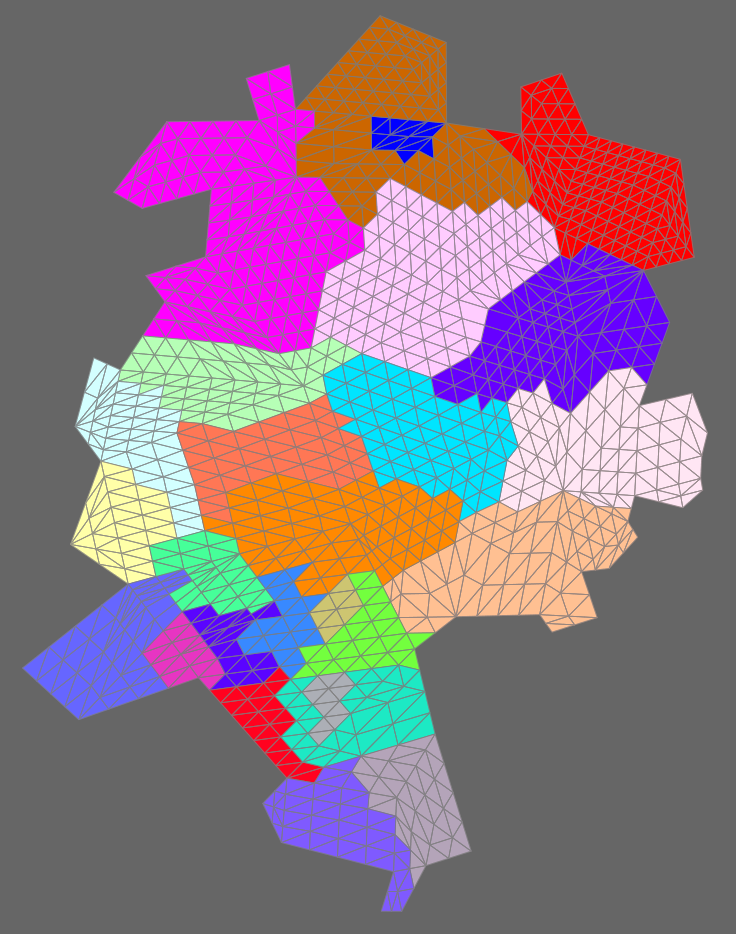
\includegraphics[width=\textwidth]{./figures/grid.png}
		\end{subfigure}
		% ---------------------
		\begin{subfigure}[b]{0.4\textwidth}
			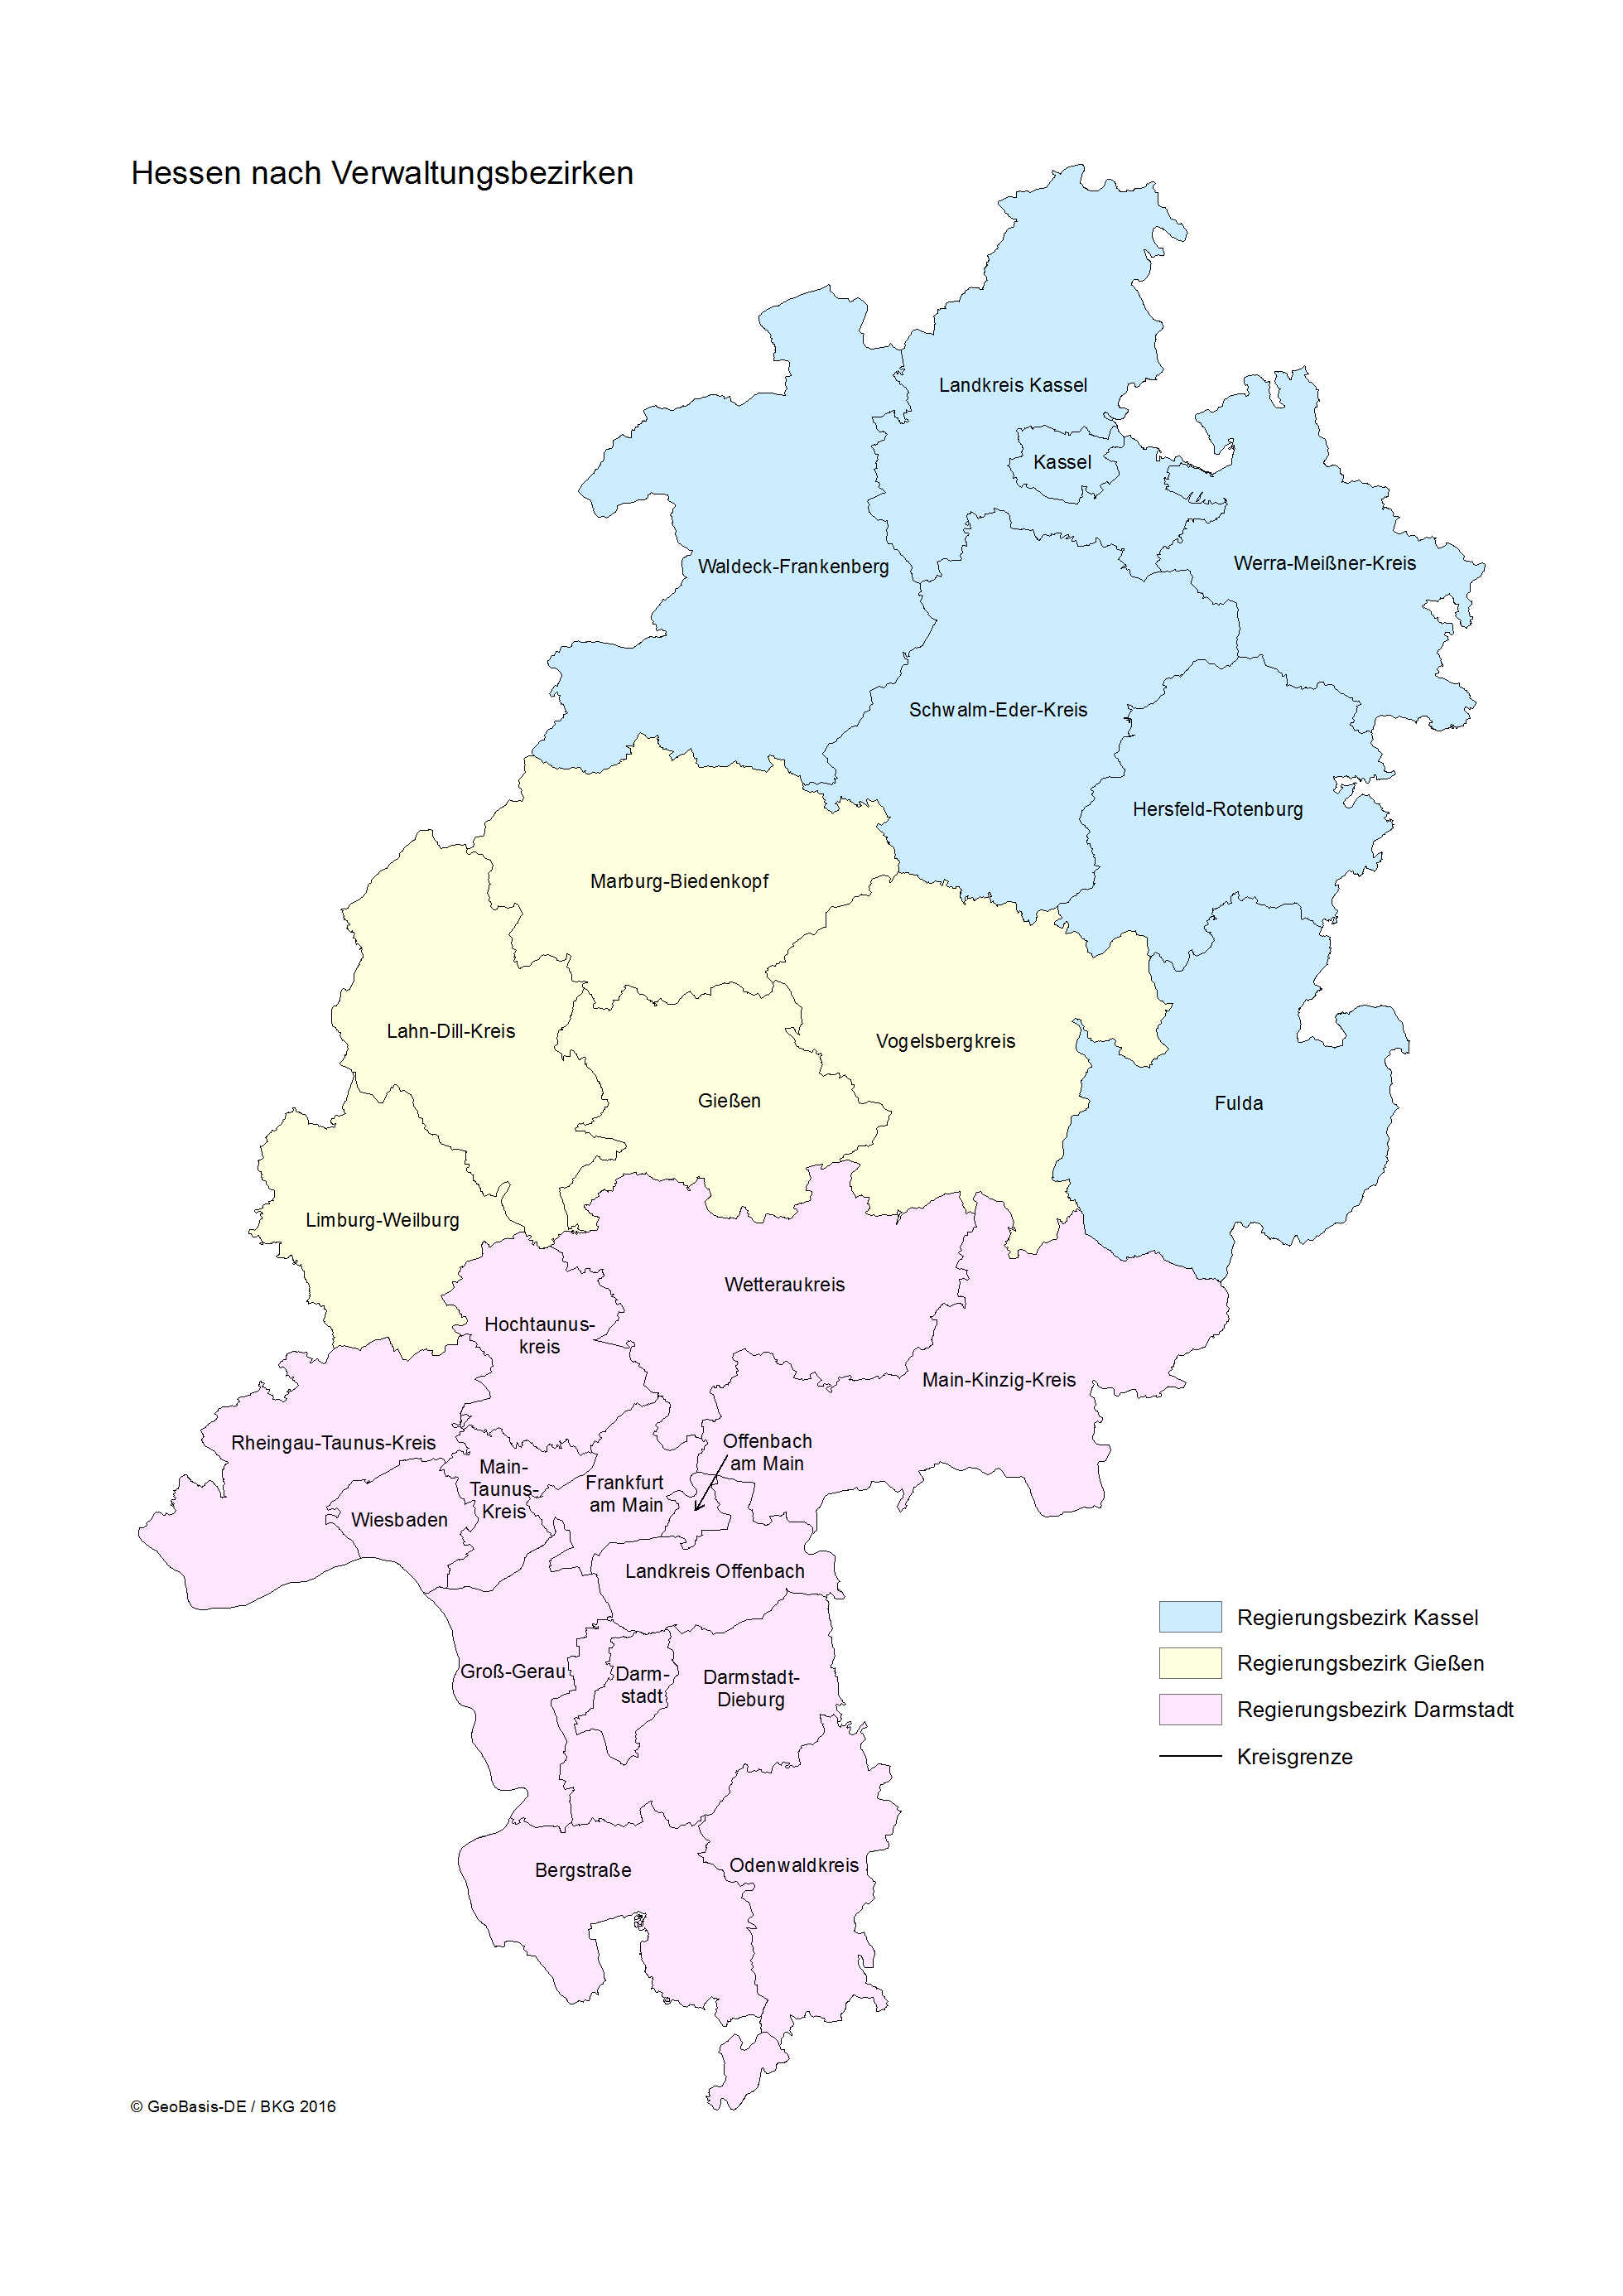
\includegraphics[width=\textwidth]{./figures/Hessen.png}
		\end{subfigure}
	\end{center}
	\caption{2d-grid of the region of Hesse. The grid consists of 1075 vertices, 3049 edges and 1975 faces.
		Each color on the grid represents a different region within Hesse. An image of Hesse is shown
		for better comparability\cite{HesseImage}.}
	\label{fig:2d-grid}
\end{figure}


%----------------------------------------------------------------------------------------
%	SECTION 3
%----------------------------------------------------------------------------------------

\section{SEIRD simulation}

\subsection{Inherited SEIRD model implementation}
The experiments of this work were  performed using the model implementation previously established in and kindly provided by
Rastogi et al.\cite{Rastogi}. The code provided included a functional implementation of the UG4 'EpidemicsRunner', as well as
the epidemics\_app folder used for  the previously mentioned project. The code was manly lua based and served as a base
for modifications and additional features added during this work. Changes and additions included both streamlining the simulation process, as
well as setting up the simulation experiments used to generate the results. The base file used to run the SEIRD simulation was epidemics.lua,
which was originally written by Prof. Gabriel Wittum and Dr. Arne N\"agel, and later modified by Devansh Rastogi and Tristan Scheidemann.
The previously mentioned lua files serve as a platform for the underlying UG4 framework. Commands issued in the lua files
are read and execute associated commands defined in UG4. 

\subsection{Process sequence of SEIRD simulations}
Simulations were performed as previously described by Rastogi et al.\cite{Rastogi}.
The implemented SEIRD simulation is based on an ugx file, that describes the geometry of the simulated regions. The file is provided
by the user and contains a number of vectors and edges. Vectors are grouped together to form regions, while edges describe possible
interactions between vectors that can be used to simulate migration between vectors. When the SEIRD model is started, starting conditions
defined in the lua code are applied to specific regions of the grid. From there the simulation is run for each
vector and the results are saved in an output file. If parameter optimization is performed, the results are then modified and processed
using the \I{ConstrainedOptimization} plugin (see \hyperref[sec:post_proc]{section \ref*{sec:post_proc}} for details).

%\subsection{LIMEX scheme}
% found new source, see notes.txt in /bachelor/thesis/

\subsection{Variable optimization}
For the process of optimizing the partial differential equation (PDE) problem, given by the model, two different solving methods
were used. The first method was a \I{Gauss-Newton} algorithm, the second was a \I{Particle Swarm Optimization} (PSO) algorithm.
During the experimental phase of the project both methods were used to investigate the questions answered in this work.
PSO was first used to roughly estimate possible target values, while \I{Gauss-Newton} was used to refine the previous findings.
Event though both methods yielded similar results in the end, all data presented in the result section of this work were created
using the \I{Gauss-Newton} algorithm. 

%----------------------------------------------------------------------------------------
%	SECTION 4
%----------------------------------------------------------------------------------------
\section{Data post-processing and variable optimization}
\label{sec:post_proc}
In order to optimize simulation results, the variables of the model equations had to be automatically adjusted based on
the loss value of the previous simulation. This section explains the steps that were undertaken to achieve this goal.

%-----------------------------------
%	SUBSECTION 1
%-----------------------------------
\subsection{Output-grid association}
The simulation results were output in the form of density values, associated with two coordinate positions ($x$ and $y$ on the
original grid). In order for the results to be processed properly, it was necessary to associate each of these
values with the correct region of the Hesse grid. To do, the program \I{geometry\_parser.lua} was written, which reads a config file,
parses and saves the positional information of each vertex in the grid and to which region it belongs. The program then compares the simulation results
with the parsed data and associates each result value with a region. Lastly the program \I{convert\_values.lua} is used to average the result values
for each region and time point, converts the average from densities to number of individuals per group and then saved the output in separate files.
One file per SEIRD group is created. The program was originally written by Devansh Rastogi and Tristan Scheidemann and later modified to
better suit the needs of this project. During simulations in which variables are optimized, the results are used to execute the program \I{ConstrainedOptimization}.


%-----------------------------------
%	SUBSECTION 2
%-----------------------------------
\subsection{Loss function}
In order to quantify the precision with which the simulation was able to reproduce the original data and optimize variables, the loss function $L$
was applied. Parameters of this function were the regions of Hesse $r$, a point in time $t$, the original data depending on
region and point in time $o(r_i,t_i)$ and the simulated data depending on region and point in time $s(r_i, t_i)$. Figure \ref*{eq:loss_newton}
shows the equation.

\textcolor{red}{do more mathematically correct}

\begin{align}
	L &= \sum_{r_0=0}^{25} \sum_{t_{0}=0}^{t} (o(r_i,t_i) - s(r_i,t_i))^{2}
	\label{eq:loss_newton}
\end{align}


%-----------------------------------
%	SUBSECTION 3
%-----------------------------------
\subsection{Variable optimization via \I{ConstrainedOptimization}}
The variables $\alpha$ and $q$ of the SEIRD system were optimized using the \I{ConstrainedOptimization} plugin for UG4\cite{Scheidemann}.
The plugin was used to optimize these variables using both the \I{Gauss-Newton} algorithm and PSO.

%Step sizes for individual time points were adjusted while using the \I{Gauss-Newton} algorithm. This was done via the Frank-Wolf algorithm\cite{Rastogi,frank-wolf}. %note add citaions


%-----------------------------------
%	SUBSECTION 4
%-----------------------------------
\subsection{Geometry sampling}
In order to better understand the sensitivity of the model for different variables, geometry sampling was done. This means that a set range for the
investigated variables was chosen and simulations were performed with randomly chosen values for said variables. After each run the total
loss of the simulation attempt was calculated and recorded. This data was then used to create a topographic map of the relation between variables
and the total loss of the simulation. In this work we observed the relation between loss and the variables $\alpha$ and $q$. These variables
were chosen, as they are the two variables influencing the observed group \B{S}. The program used for this task was the \I{geometry\_sampler}
provided in \I{ConstrainedOptimization}.


%----------------------------------------------------------------------------------------
%	SECTION 4
%----------------------------------------------------------------------------------------
\section{Data evaluation}
Data analysis of the simulation results was one of the main parts of this work. This section will highlight techniques and tools used during this process.

%-----------------------------------
%	SUBSECTION 1
%-----------------------------------
\subsection{Box plots}
Presenting the amount of data that was acquired in a compact and presentable way proved to be challenging. We decided to use box plots
as one of the main methods of presenting our data, as they convey a lot of key information to the reader without being to overwhelming.
Each box plot is made up of multiple elements. A Minimum, a Maximum, a first Quartile (Q1), a third Quartile (Q3), the Median and
the Outliers of the measurement. The Median is the middle value of the entire data set and lies between Q1 and Q3. Q1  is the Median 
between the lowest value of the data set and the Median of the entire data set. Thus 25\% of all data points are below and 75\% of
all data points are above Q1. Reversely Q3 is the Median value between the Median and the
highest value of the entire data set. Thus 75\% of all data ponints are below and 25\% of all data points are above Q3.
The difference between Q1 and Q3 is called the interquartile range (IQR). The Minimum and Maximum are
defined as $\text{Minimum} = Q1 - x*\text{IQR}$ and $\text{Maximum} = Q3 + x*\text{IQR}$, where $x$ was set to 1.5.
All values in the data set, that are located outside of the Minimum or Maximum are called Outliners and are represented as circles.
\hyperref[fig:boxplot]{Figure \ref*{fig:boxplot}} summarizes these definitions in an image.

\begin{figure}
	\begin{center}
		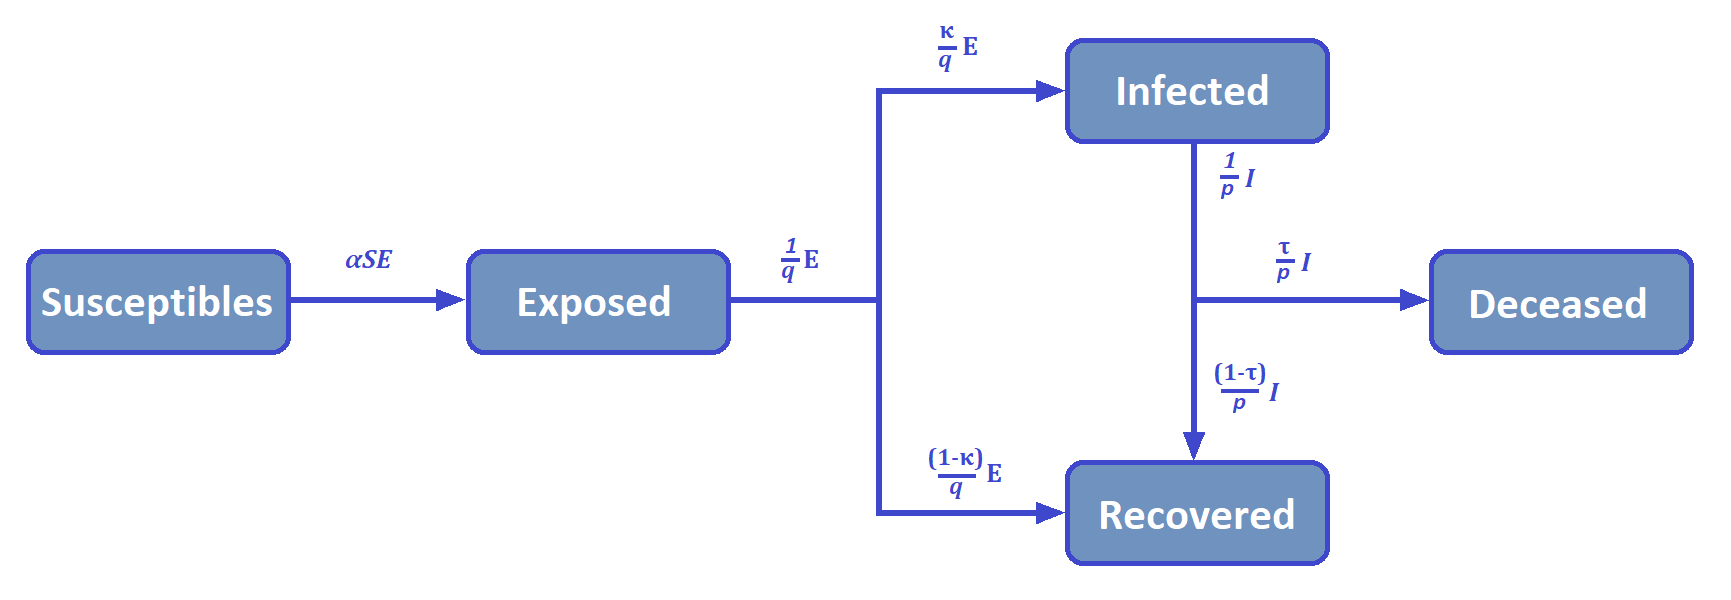
\includegraphics[width=0.75\textwidth]{./figures/SEIRD.png}
		\caption{Exemplary illustration of a box plot.
			}
		\label{fig:boxplot}
	\end{center}
\end{figure}


%-----------------------------------
%	SUBSECTION 2
%-----------------------------------
\subsection{Custom programs}
In order to present the results three custom programs were written. \I{deviation\_graph.py} was used to compare the data points of
individual regions. Graphs were created using matplotlib and numpy. Shortened data sets were extrapolated by fitting a polynomial
of degree three to the simulated data points. The resulting function was then extrapolated in order to highlight trends of the
analyzed data set. \I{deviation\_boxplot.py} was used to create box plots and \I{sensitivity\_plot} was used to visualize the
relation between $\alpha$, $q$ and the loss function in a three dimensional graph.

% Chapter Template

\chapter{Results} % Main chapter title
\textcolor{red}{add short explanations when first mentioning $\alpha$ and $q$ as reminder}

\label{chap:results} % Change X to a consecutive number; for referencing this chapter elsewhere, use \ref{ChapterX}
This chapter will summarize the results of this work. First, the results of simulating the susceptible population
in the region of Hesse will be presented. Then the results of a sensitivity analysis for the variables $\alpha$ and
$q$ will be shown. Specifically the sensitivity analysis will later be used in \hyperref[chap:discussion]{Chapter
\ref*{chap:discussion} - Discussion} to explain the results of the simulations.


%----------------------------------------------------------------------------------------
%	SECTION 1
%----------------------------------------------------------------------------------------

\section{Simulating the susceptible population of Hesse}
\label{sec:sim_res}
\textcolor{red}{check your tenses and make sure they make sense!}
\textcolor{red}{remove data point/day inconsistencies}

During this work we simulated the susceptible population of Hesse. 26 regions were simulated over a time period of
76, 60 and 50 days respectively. We will present both the absolute and percentage difference between the simulated
and the original data for each time frame.

\textcolor{red}{redo box plots with x-axis description}
\textcolor{red}{ADD OPTIMAL VALUES FOR $\alpha$ AND $q$!!}
%-----------------------------------
%	SUBSECTION 1
%-----------------------------------
\subsection{Simulating susceptibles in a 76 day time frame}
We first wanted to observe how well the simulation performs in a time frame of 76 days. Since the number of susceptible
individuals is much greater then any other group at any given data point, changes in this group can be difficult to
observe. Because of this we decided to calculate and compare the number of individuals that migrated from the susceptible
to the exposed group instead. This was done by subtracting the number of susceptible individuals at data point \I{t=x} from
the start point \I{t=0}. The result is the total change of susceptibles at any given time point, which is equivalent to the 
sum of all exposed individuals at any given time point. These results are much easier to compare and understand.
\hyperref[fig:76_sim_expl]{figure \ref*{fig:76_sim_expl}} shows three graphs that illustrate this process.


\begin{figure}
	\centering
	\begin{subfigure}[b]{0.3\textwidth}
		\centering
		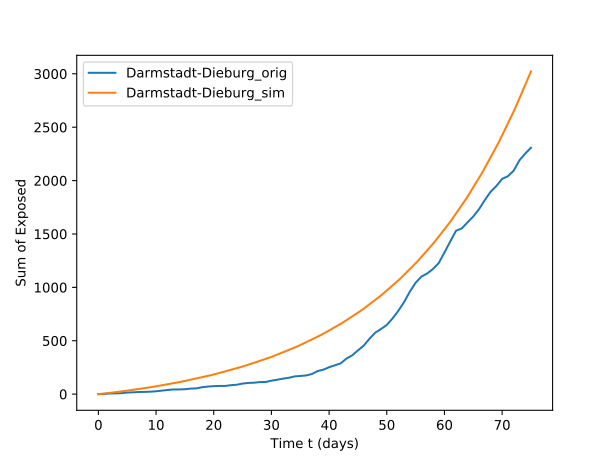
\includegraphics[width=\textwidth]{./figures/76d/24_Darmstadt-Dieburg.png}	
		\caption{}
	\end{subfigure}
	\hfill
	\begin{subfigure}[b]{0.3\textwidth}
		\centering
		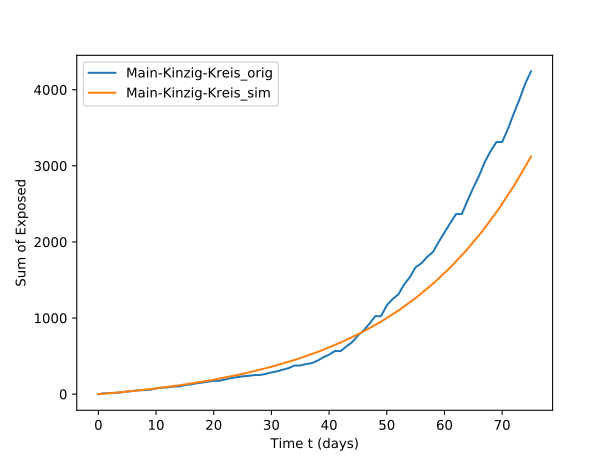
\includegraphics[width=\textwidth]{./figures/76d/13_Main-Kinzig-Kreis.png}	
		\caption{}
	\end{subfigure}
	\hfill
	\begin{subfigure}[b]{0.3\textwidth}
		\centering
		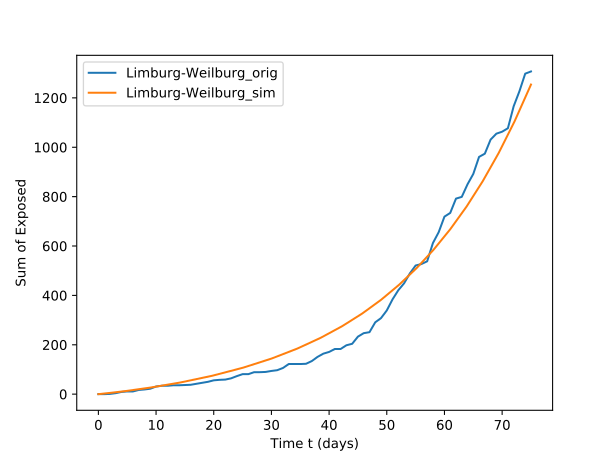
\includegraphics[width=\textwidth]{./figures/76d/10_Limburg-Weilburg.png}	
		\caption{}
	\end{subfigure}
	\caption{Three exemplary results of a simulation of the exposed individuals.
		The original (``orig'') data is drawn in blue and the simulated (``sim'') data is drawn in orange.
		The number of simulated exposed individuals can be greater (image (A), region ``Darmstadt Dieburg''), smaller 
		(image (B), region ``Mein Kinzig Kreis'') or about the same (image (C), region ``Limburg Weilburg''), as 
		the originally observed number of exposed.
		}
	\label{fig:76_sim_expl}
\end{figure}

Furthermore we analyzed the percentage deviation of original and simulated data for each time step in each region. The results
are shown in a box plot in \hyperref[fig:76_sim_box]{figure \ref*{fig:76_sim_box}}. The three regions ``Werra-Meissner-Kreis'',
``Marburg-Biedenkopf'' and ``Limburg-Weilburg'' are listed separately in figure \ref*{fig:76_sim_box}, in order to make the scales
more readable.


\begin{figure}
	\centering
	\begin{subfigure}[b]{0.4\textwidth}
		\centering
		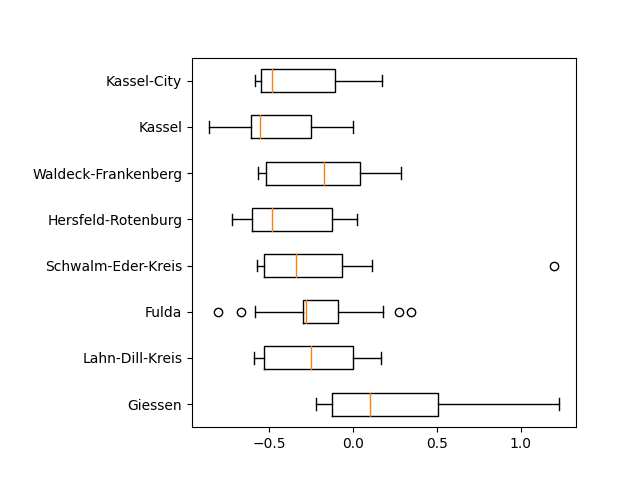
\includegraphics[width=\textwidth]{./figures/76d/deviation_box76_alt1.png}	
	\end{subfigure}
	\begin{subfigure}[b]{0.4\textwidth}
		\centering
		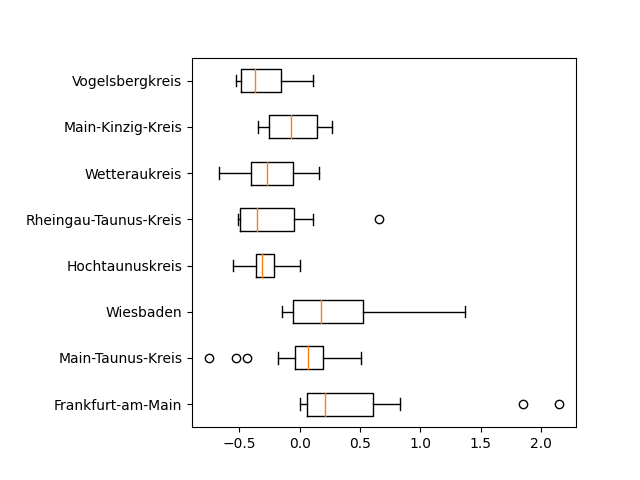
\includegraphics[width=\textwidth]{./figures/76d/deviation_box76_alt2.png}	
	\end{subfigure}
	\begin{subfigure}[b]{0.4\textwidth}
		\centering
		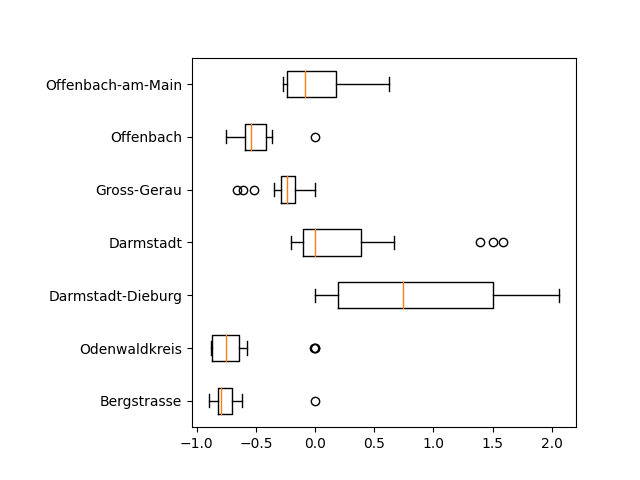
\includegraphics[width=\textwidth]{./figures/76d/deviation_box76_alt3.png}	
	\end{subfigure}
	\begin{subfigure}[b]{0.4\textwidth}
		\centering
		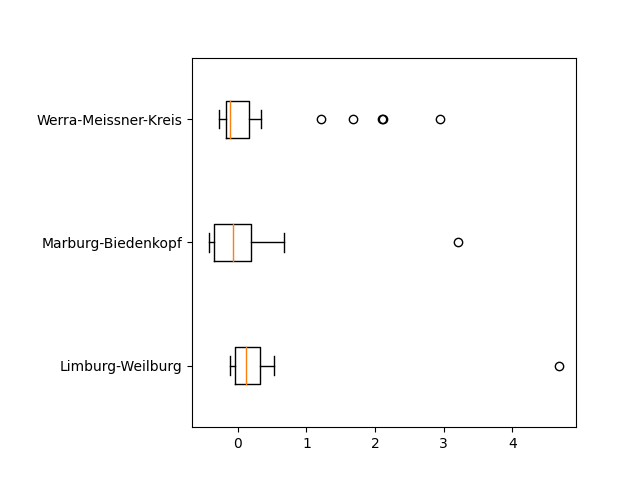
\includegraphics[width=\textwidth]{./figures/76d/deviation_box76_alt4.png}	
	\end{subfigure}
	\caption{Shown are box plots of the percentage deviation, of every simulated region relative to the original data.}
	\label{fig:76_sim_box}
\end{figure}

\textcolor{red}{rephrase for deviation factor and meaning}
Figure \ref*{fig:76_sim_box} shows that the simulated regions have a wide range of median values regarding the deviation.
The numbers are ranging between a median deviation factor of about -0.8 and +0.75. This means, that the model calculated
between 80 percent less or 75 percent more infection events, compared to the original data. 12, 21 and 25 of the 26 regions have
an absolute median deviation of less than 25, 50 and 75 percent respectively. Only the region ``Berstrasse'' had a higher deviation with
about -79.16 percent. 19 regions have a negative and 6 regions have a positive median deviation. The region ``Darmstadt'' had a
median deviation of exactly 0. Many of the plots are skewed right.
(\textcolor{red}{explain and describe better, also add data to Appendix!!!})



%-----------------------------------
%	SUBSECTION 2
%-----------------------------------
\subsection{Simulating susceptibles in a 60 day time frame}
In order to explore how well the model is working with a smaller data set, the same optimization process as in the previous section was
applied to a 60 day data set. Only the first 60 days of the previously chosen time frame were simulated, the other 16 days were
simply removed. \hyperref[fig:60_sim_expl]{Figure \ref*{fig:60_sim_expl}} shows three exemplary graphs of the simulation results.
For better comparability, the same regions were chosen as in previous section. The results were extrapolated in order to better visualize
the trend of the simulation result.

\begin{figure}
	\centering
	\begin{subfigure}[b]{0.3\textwidth}
		\centering
		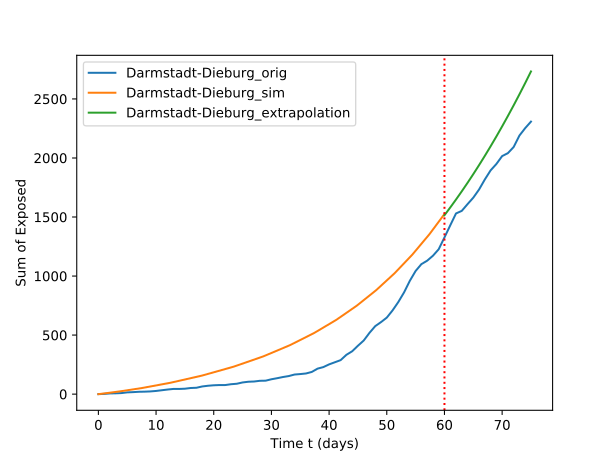
\includegraphics[width=\textwidth]{./figures/60d/24_Darmstadt-Dieburg.png}	
		\caption{}
	\end{subfigure}
	\hfill
	\begin{subfigure}[b]{0.3\textwidth}
		\centering
		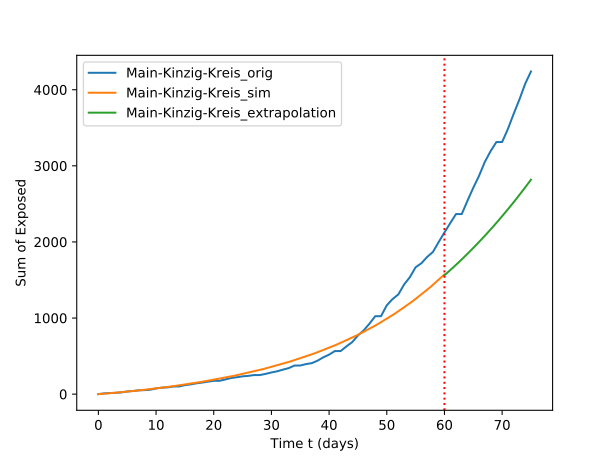
\includegraphics[width=\textwidth]{./figures/60d/13_Main-Kinzig-Kreis.png}	
		\caption{}
	\end{subfigure}
	\hfill
	\begin{subfigure}[b]{0.3\textwidth}
		\centering
		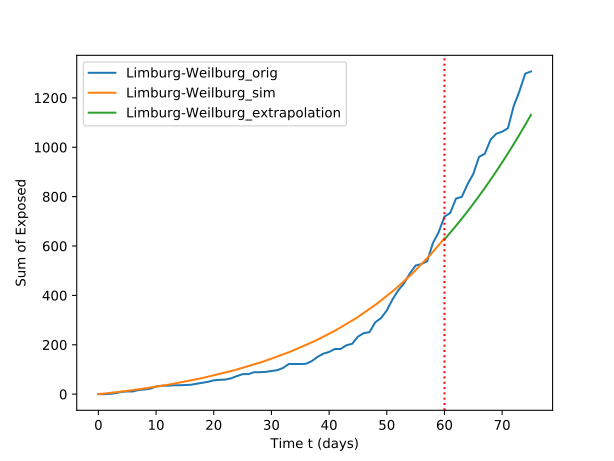
\includegraphics[width=\textwidth]{./figures/60d/10_Limburg-Weilburg.png}	
		\caption{}
	\end{subfigure}
	\caption{Three exemplary results of a simulation of the exposed individuals. The original (``orig'') data is drawn in blue,
		the simulated (``sim'') data is drawn in orange and the extrapolation of the simulated data (``extrapolation'') is
		drawn in green. The vertical red dotted line marks the transition from simulated to extrapolated data.
		}
	\label{fig:60_sim_expl}
\end{figure}

Figure \ref*{fig:60_sim_expl} shows that the general trend of the simulations remains similar to the simulations with 76 data points.
In all three regions, the extrapolated data points show a slightly slower increase in infections compared to the simulations
with 76 days in figure \ref*{fig:76_sim_expl}.

Similar to the previous section, we calculated the deviation of each data point for
each region and expressed the results in a set of box plots. The results are shown in figure \ref*{fig:60_sim_box}. Only data points
that were actually simulated were included into this analysis. Extrapolated data points were not used.

\textcolor{red}{more text for box plots}



\begin{figure}
	\centering
	\begin{subfigure}[b]{0.4\textwidth}
		\centering
		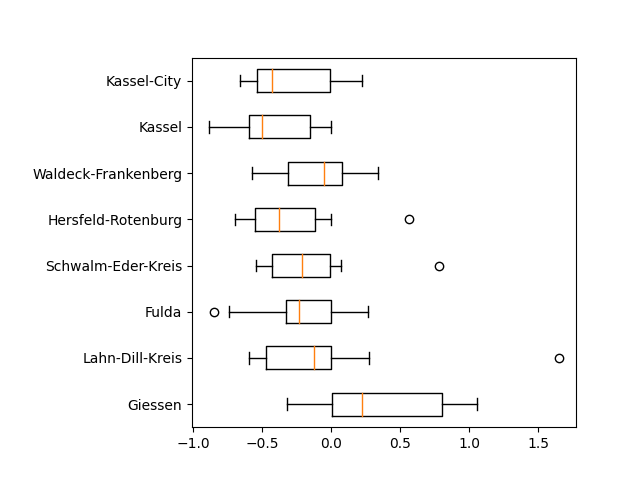
\includegraphics[width=\textwidth]{./figures/60d/deviation_box60_alt1.png}	
	\end{subfigure}
	\begin{subfigure}[b]{0.4\textwidth}
		\centering
		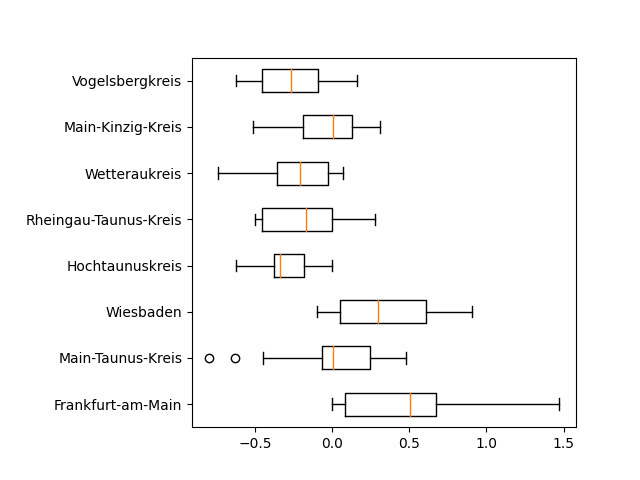
\includegraphics[width=\textwidth]{./figures/60d/deviation_box60_alt2.png}	
	\end{subfigure}
	\begin{subfigure}[b]{0.4\textwidth}
		\centering
		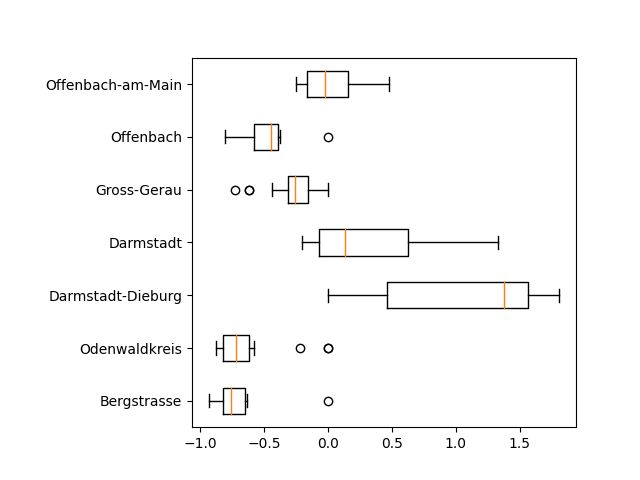
\includegraphics[width=\textwidth]{./figures/60d/deviation_box60_alt3.png}	
	\end{subfigure}
	\begin{subfigure}[b]{0.4\textwidth}
		\centering
		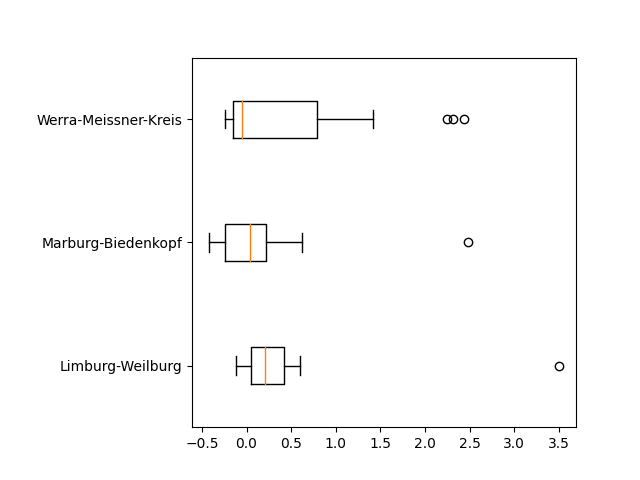
\includegraphics[width=\textwidth]{./figures/60d/deviation_box60_alt4.png}	
	\end{subfigure}
	\caption{Shown are box plots of the percentage deviation, of every simulated region relative to the original data.
		In this experiment only 60 of 76 data points were used to simulate the original data. The median of all
		simulated regions ranges between -0.76 and 1.38 and the median interquartile range is 0.41. 19 regions
		have a negative and 6 regions have a positive median deviation. The three regions ``Werra-Meissner-Kreis'',
		``Marburg-Biedenkopf'' and ``Limburg-Weilburg'' are shown separately for better scaling.
		}
	\label{fig:60_sim_box}
\end{figure}

As with the graphs described before, the deviation results of the 60 data point simulation are largely comparable to the 76
data point deviation results. The maximum and minimum median deviation of all regions is higher compared to previous results,
lying between about -76 percent and 138 percent. 14, 21 and 24 regions had an absolute, median deviation of less than
25, 50 and 75 percent respectively. The two regions with a deviation higher than 75 percent were ``Bergstrasse'' and
``Darmstadt-Dieburg'' with median deviations of -75.52 and 137.31 percent respectively.
19 of the 26 regions had a negative and 6 of the 26 regions had a positive median deviation.
As in the previous section many box plots are skewed to the right, however this effect seems to be less prominent then in
the 76 data point simulation.


%-----------------------------------
%	SUBSECTION 3
%-----------------------------------
\subsection{Simulating susceptibles in a 50 day time frame}
The last simulation that was performed, was a simulation with 50 data points. As described in the previous section with
60 data points, simulations and optimization steps were performed on a truncated data set, where the last 26 of the total
76 data points were removed. \hyperref[fig:50_sim_expl]{Figure \ref*{fig:50_sim_expl}} shows three exemplary graphs of this
experiment. As previously, the same regions were chosen as for the 76 data point experiment. 
\textcolor{red}{add more explanation and description once graphs are there}

\begin{figure}
	\centering
	\begin{subfigure}[b]{0.3\textwidth}
		\centering
		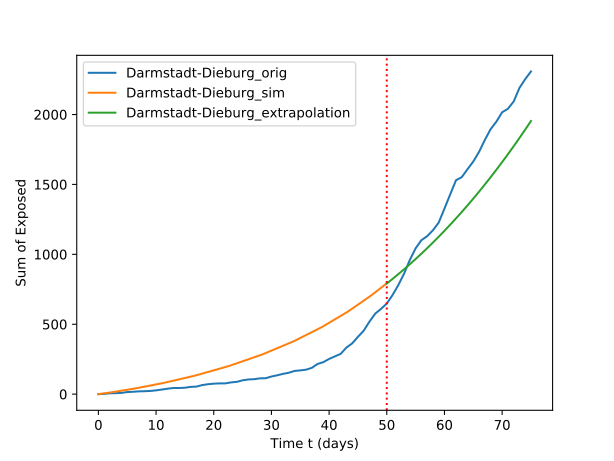
\includegraphics[width=\textwidth]{./figures/50d/24_Darmstadt-Dieburg.png}	
		\caption{}
	\end{subfigure}
	\hfill
	\begin{subfigure}[b]{0.3\textwidth}
		\centering
		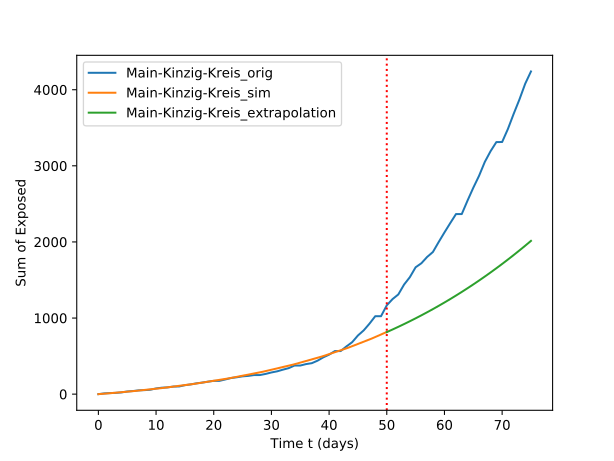
\includegraphics[width=\textwidth]{./figures/50d/13_Main-Kinzig-Kreis.png}	
		\caption{}
	\end{subfigure}
	\hfill
	\begin{subfigure}[b]{0.3\textwidth}
		\centering
		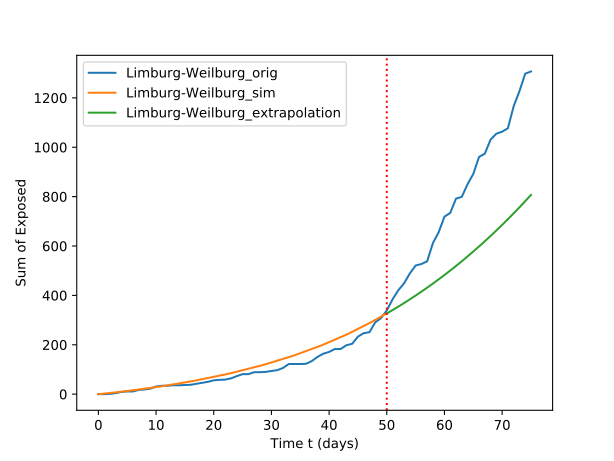
\includegraphics[width=\textwidth]{./figures/50d/10_Limburg-Weilburg.png}	
		\caption{}
	\end{subfigure}
	\caption{Add caption
		}
	\label{fig:50_sim_expl}
\end{figure}
In this experiment all three
regions show a stronger trend towards a negative deviation compared to the previous two experiments. While the regions of
the graphs, that were simulated based on the provided data points, looks similar, the overall trend visualized by
the extrapolation shows a strong deviation towards to little infections.

As with the 60 data point analysis, we also performed the deviation analysis on the 50 data point data set. As previously described
only actually simulated data points were included into the analysis. Extrapolated data points were not used. The results of this
analysis are shown in \hyperref[fig:50_sim_box]{Figure \ref*{fig:50_sim_box}}.

\begin{figure}
	\centering
	\begin{subfigure}[b]{0.4\textwidth}
		\centering
		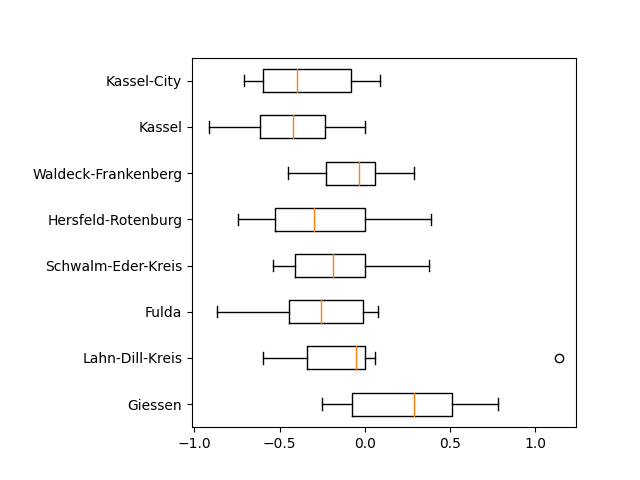
\includegraphics[width=\textwidth]{./figures/50d/deviation_box50_alt1.png}	
	\end{subfigure}
	\begin{subfigure}[b]{0.4\textwidth}
		\centering
		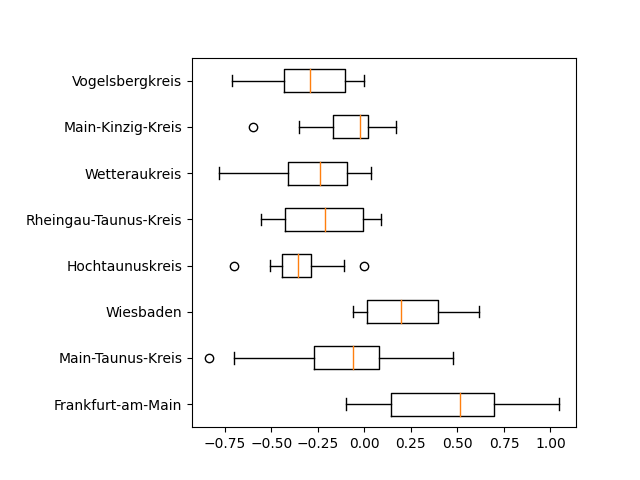
\includegraphics[width=\textwidth]{./figures/50d/deviation_box50_alt2.png}	
	\end{subfigure}
	\begin{subfigure}[b]{0.4\textwidth}
		\centering
		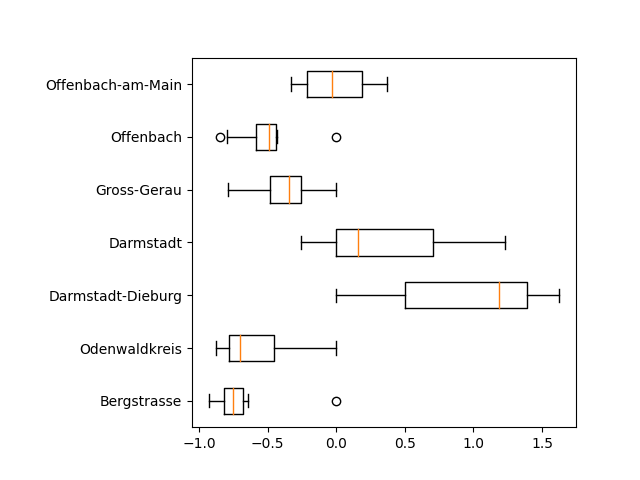
\includegraphics[width=\textwidth]{./figures/50d/deviation_box50_alt3.png}	
	\end{subfigure}
	\begin{subfigure}[b]{0.4\textwidth}
		\centering
		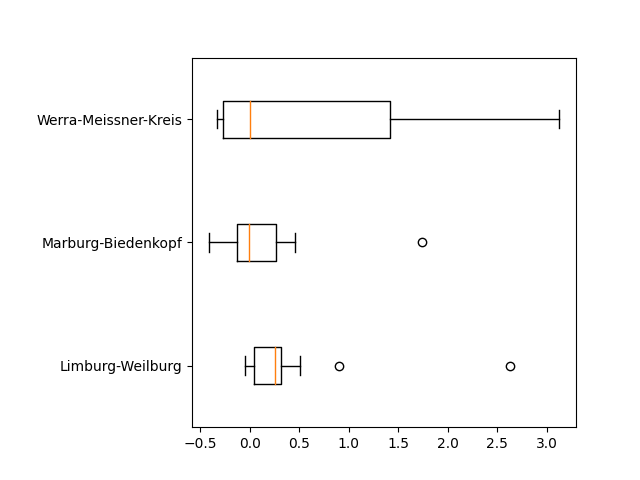
\includegraphics[width=\textwidth]{./figures/50d/deviation_box50_alt4.png}	
	\end{subfigure}
	\caption{Shown are box plots of the percentage deviation for a simulated time frame of 50 days. Each box plot includes
		all percentage deviations of all simulated data points compared to the original data. The median of all regions
		ranges between -0.76 and 1.19 and the median interquartile range is 0.38. 19 regions had a positive and
		6 regions had a negative median deviation. One region had a median deviation of exactly 0.
		The three regions ``Werra-Meissner-Kreis'', ``Marburg-Biedenkopf'' and ``Limburg-Weilburg'' are shown
		separately for better scaling.
		}
	\label{fig:50_sim_box}
\end{figure}

The 50 data point simulations show similar results to the previous two experiments. The median deviation of all regions
ranges between -76 and +119 percent and the median interquartile range is 0.38. 12, 22 and 24 regions out of 26 have an
absolute median deviation of less then 25, 50 and 75 percent respectively. The two region with a higher median
deviations are ``Bergstrasse'' and ``Darmstadt-Dieburg'', with -75.56 and 118.36 percent deviation respectively.
The skew of the box plots however is not as uniform. Many plots are skewed right like in the previous experiments, but
there is also an increased number of blots with a skew to the left. 19 of the 26 regions had a negative median deviation,
6 had a positive median deviation and one region had a median deviation of exactly 0.


%----------------------------------------------------------------------------------------
%	SECTION 2
%----------------------------------------------------------------------------------------

\section{Influence of individual regions on the loss function}
In order to better understand the influence of individual regions on the model itself, we manually calculated the total
loss, the individual loss for each region and the percentage loss of each region relative to the total loss.
\hyperref[tab:perc_region_loss]{Table \ref*{tab:perc_region_loss}} shows the results of these calculations. The table
is sorted descending from highest to lowest percentage loss contribution.
\textcolor{red}{add table with total information to Appendix}

\begin{table}
	\caption{the caption}
	\begin{tabular}{|l|x{2cm}|x{2cm}|x{2cm}|}
	%\begin{tabular}{|l|c|c|c|}
		\hline
		\B{region} & \B{percentage loss} & \B{percentage population} & \B{median deviation} \\ \hline \hline
		Offenbach & 27.70 & 5.67 & -0.54 \\ \hline
		Bergstrasse & 14.41 & 4.31 & -0.79 \\ \hline
		Frankfurt-am-Main & 13.10 & 12.14 & 0.21 \\ \hline
		Lahn-Dill-Kreis & 6.29 & 4.03 & -0.25 \\ \hline
		Main-Kinzig-Kreis & 5.17 & 6.70 & -0.07 \\ \hline
		Marburg-Biedenkopf & 4.70 & 3.91 & -0.06 \\ \hline
		Kassel-City & 3.90 & 3.19 & -0.49 \\ \hline
		Wetteraukreis & 3.35 & 4.93 & -0.27 \\ \hline
		Gross-Gerau & 2.90 & 4.38 & -0.23 \\ \hline
		Rheingau-Taunus-Kreis & 2.89 & 2.98 & -0.36 \\ \hline
		Kassel & 2.58 & 3.77 & -0.55 \\ \hline
		Hochtaunuskreis & 2.33 & 3.77 & -0.32 \\ \hline
		Darmstadt-Dieburg & 2.00 & 4.73 & 0.74 \\ \hline
		Odenwaldkreis & 1.93 & 1.54 & -0.75 \\ \hline
		Offenbach-am-Main & 1.23 & 2.08 & -0.09 \\ \hline
		Schwalm-Eder-Kreis & 1.03 & 2.86 & -0.34 \\ \hline
		Waldeck-Frankenberg & 0.99 & 2.49 & -0.17 \\ \hline
		Giessen & 0.84 & 4.32 & 0.10 \\ \hline
		Wiesbaden & 0.80 & 4.43 & 0.17 \\ \hline
		Fulda & 0.74 & 3.54 & -0.28 \\ \hline
		Hersfeld-Rotenburg & 0.41 & 1.91 & -0.48 \\ \hline
		Main-Taunus-Kreis & 0.25 & 3.80 & 0.07 \\ \hline
		Darmstadt & 0.18 & 2.53 & 0.00 \\ \hline
		Vogelsbergkreis & 0.17 & 1.68 & -0.37 \\ \hline
		Limburg-Weilburg & 0.08 & 2.74 & 0.11 \\ \hline
		Werra-Meissner-Kreis & 0.03 & 1.59 & -0.11 \\ \hline
	\end{tabular}
	\label{tab:perc_region_loss}
\end{table}

The results show, that the main contribution of the loss function is done by a minority of regions. The top three contributors
account for 55.21 percent of the entire loss, while only making up about 22.12 percent of the total population. The top seven
contributors make up about 75.27 percent, while making up about 39.95 percent of the population. A notable find is, that the
top two regions, ``Offenbach'' and ``Bergstrasse'', both display a negative deviation, while the third most influential region
``Frankfurt-am-Main'' has a positive deviation. Frankfurt also has a lower overall contribution to the loss, than the other
two regions, even though it has a higher share of the total population then the other two regions combined.

%----------------------------------------------------------------------------------------
%	SECTION 3
%----------------------------------------------------------------------------------------

\section{Sensitivity analysis of $\alpha$ and $q$}
\textcolor{red}{add more angles to the images}
In order to further investigate the features of the model, we analyzed the sensitivity of the loss function relative to
the variables $\alpha$ and $q$. We only chose those two variables, since the loss function was only calculated based
on the difference between the simulated and the original susceptible population. Since this group only depends on those
two variables in our model, changes in the other variables could not influence the loss and were therefore not investigated.
For this experiment, the 4000 simulations of the model with all 76 original data points were performed and the variables
$\alpha$ and $q$ were chosen randomly, within a set constraint. The upper and lower bounds were set to 0.05 and 0.35 for 
$\alpha$ and 5.5 and 8.0 for $q$ respectively. The results of these simulations were gathered and used to plot a map
of the variable landscape of the loss of the susceptible group.
\hyperref[fig:sensitivity_zoom0]{Figure \ref*{fig:sensitivity_zoom0}} shows the total result of all simulations over the
chosen bounds.

\begin{figure}
	\centering
	\begin{subfigure}[b]{0.4\textwidth}
		\centering
		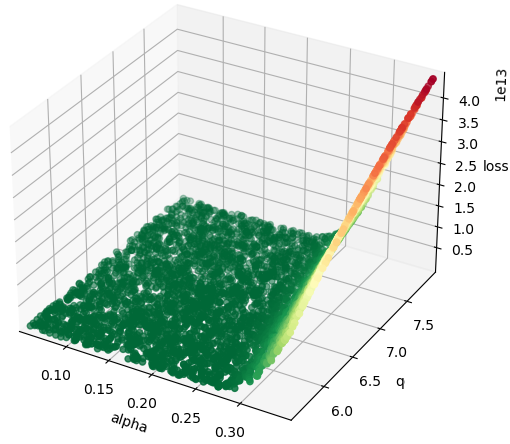
\includegraphics[width=\textwidth]{./figures/sensitivity/sensitivity_zoom0_0_2.png}	
	\end{subfigure}
	\begin{subfigure}[b]{0.4\textwidth}
		\centering
		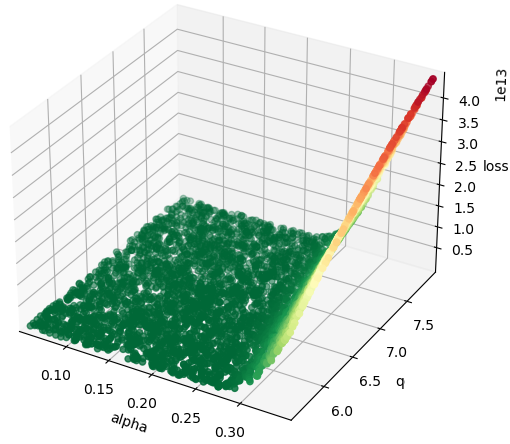
\includegraphics[width=\textwidth]{./figures/sensitivity/sensitivity_zoom0_0_2.png}	
	\end{subfigure}
	\caption{Visualization of the variable sensitivity of the susceptible group. The variables $\alpha$ and $q$ were plotted
		against the loss of the susceptible group. Images (A) and (B) show the plot from different angles in order
		to increase readability. In the model the susceptible group shows sensitivity to changes of both $\alpha$ and
		$q$. However, the sensitivity to $q$ seems to be dependent on $\alpha$.
		}
	\label{fig:sensitivity_zoom0}
\end{figure}

\textcolor{red}{add result values to figure explanation}
Figure \ref*{fig:sensitivity_zoom0} shows that low values for $\alpha$ lead to a decreased sensitivity of the loss function
for $q$. Only after an $\alpha$ value of about 0.25 is reached, does the loss start to react to changes in $q$. After this point
however, the loss function quickly increases. This phenomenon can be seen both, if $q$ is increased and if $q$ is not increased
in the simulation. But a bigger $q$ value causes the loss to increase more quickly compared to a simulation with a small loss.



The simulations were further investigated by plotting only part of the experimental data.
The first row of \hyperref[fig:sensitivity_zoom0]{Figure \ref*{fig:sensitivity_zoom0}} shows all data points with $\alpha$ values between 0.15
and 0.25, $q$ values between 5.5 and 8.0 and a maximum loss of $10^{10}$. The loss on this image was capped in order to reduce
the scale of the loss and thereby increase readability. This lead 957 of 4000 data points being plotted. The images in the
second row show the same graph (\textcolor{red}{?}), with the same bonds for $\alpha$ and $q$, but with a maximum loss capped
at $2.7*10^{9}$. This gives an even closer look at the range of optimal/close-to-optimal values for $\alpha$ and $q$.

\begin{figure}
	\centering
	\begin{subfigure}[b]{0.4\textwidth}
		\centering
		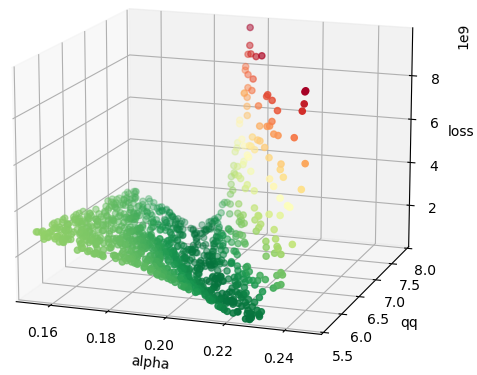
\includegraphics[width=\textwidth]{./figures/sensitivity/sensitivity_zoom1_0_2.png}	
	\end{subfigure}
	\begin{subfigure}[b]{0.4\textwidth}
		\centering
		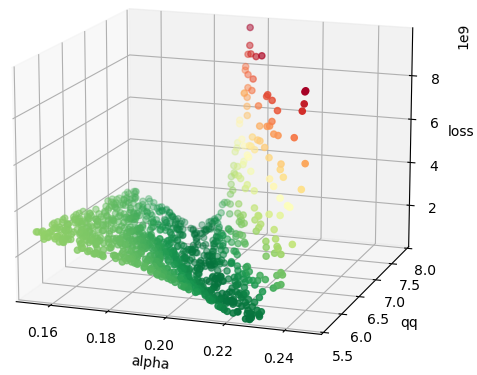
\includegraphics[width=\textwidth]{./figures/sensitivity/sensitivity_zoom1_0_2.png}	
	\end{subfigure}
	\begin{subfigure}[b]{0.4\textwidth}
		\centering
		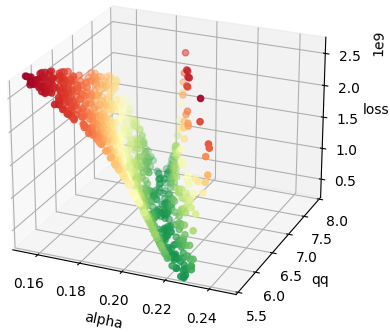
\includegraphics[width=\textwidth]{./figures/sensitivity/sensitivity_zoom2_0_2.png}	
	\end{subfigure}
	\begin{subfigure}[b]{0.4\textwidth}
		\centering
		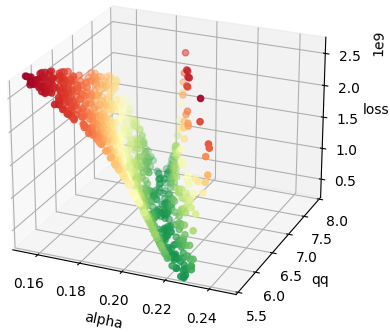
\includegraphics[width=\textwidth]{./figures/sensitivity/sensitivity_zoom2_0_2.png}	
	\end{subfigure}
	\caption{Visualization of the variable sensitivity of the susceptible group. The variables $\alpha$ and $q$ were
		capped to 0.15 and 0.25 and 5.5 and 8.0 respectively and then plotted against the result of the loss function.
		The loss was capped at $10^{10}$ and $2.7*10^{9}$ for the first and the second row respectively, in order to
		reduce the scale of the loss and make the image more readable. The image shows that there seems to be a set of
		optimal value combinations of $\alpha$ and $q$, where the loss is minimized. Given the diagonal nature of this
		``optimal cavity'' there seem to be an equilibrium between the two values.
		\textcolor{red}{check for better wording} %note
		}
	\label{fig:sensitivity_zoom1}
\end{figure}

Figure \ref*{fig:sensitivity_zoom1} shows the existence of a ``valley'' with minimized loss. It can be seen that there are 
sets of values of $\alpha$ and $q$, where the loss appears to be minimized. The optimal values found by the model for $\alpha$
and $q$ are also withing this region (\textcolor{red}{more info}). The optimized area seems to have a diagonal structure,
indicating an optimal relation between $\alpha$ and $q$.


% Chapter Template

\chapter{Discussion} % Main chapter title
\label{chap:discussion} % Change X to a consecutive number; for referencing this chapter elsewhere, use \ref{ChapterX}
\textcolor{red}{weave in story, why only susceptibles were examined in experiments!}

This chapter will summarize, discuss and interpret the results of the \hyperref[chap:results]{previous section
\ref*{chap:results}}. We will start by discussing and evaluating the accuracy of the model regarding the reproduction
of real world data, as the ability to predict future outcomes with fewer data points. After that, we will use the
analyze the results of the loss function analysis and the sensitivity analysis in order to better understand the results
and identify potential issues and areas of improvement. Lastly an outlook will be given for possible strategies and
ideas to improve both the implementation of the model and the model itself.
%----------------------------------------------------------------------------------------
%	SECTION 1
%----------------------------------------------------------------------------------------

\section{Simulation results and sensitivity analysis}
The following section will discuss the results of the simulations, the optimization process as well as the sensitivity
analysis performed in this context.
\textcolor{red}{add more text?}


%-----------------------------------
%	SUBSECTION 2
%-----------------------------------
\subsection{Simulation accuracy and optimization issues}
\hyperref[sec:sim_res]{Section \ref*{sec:sim_res}} has presented the simulation results produced by the current implementation
of the SEIRD model. It can be seen, that the accuracy of the simulation somewhat depends on the amount of data points supplied.
While the median susceptible deviation of all regions ranged between -80 and +140 percent, most the regions showed reasonable
amounts of deviation from the original data. In case of the 76 data point simulation, 21 of 26 regions showed an
absolute median deviation of 50 percent or less. Similar behavior was observed for the 60 and 50 data point simulations, in which
21 and 22 regions respectively showed an absolute median deviation of 50 percent or less. While the simulation accuracy of single regions
might differ between experiments (\textcolor{red}{double check this!}), results are overall comparable.\newline

Predicting the original data proved more difficult. While the calculated trend for the 60 data point experiment was comparable
to the simulation with 76 data points, the 50 data point simulation showed strong differences and proved to be mostly inaccurate.\\
\textcolor{red}{needs hard data to support these claims, check python code on how to extract data points and add to results.
Then come back and redo this}\\ %note

A consistent observation throughout all experiments was a strong trend of the simulated regions to negatively deviate from the
original data. This means that the simulations generally predicted lower amounts of exposed individuals than seen in the original
data. In all three experiments 19 of the 26 regions deviated in this way from the original data. This may seem odd at first,
since it could be expected, that the optimal state of the model is reached, when a maximum amount of regions are close to matching
their original data. However, if  closer attention if given to the way optimization was done in these experiments this phenomenon
becomes much clearer. All adjustments were done based on minimizing the loss function. The loss function itself was defined in
\hyperref[eq:loss_newton]{equation \ref*{eq:loss_newton}} as the sum of the square difference between the simulated and the original
data of all data points and each region. This means that a regions individual influence on the adjustment of model variables
increases as the total difference between its simulated and original data grows. This effect is further increased, since the
difference between original and simulated data is squared before it is summed up. Thus leading to a quadratic increase in influence
of highly deviating regions relative to the other regions. \newline

Combining this knowledge with the observations of the model results, helped us to identify three factors that can be used to explain
the optimization behavior of the current implementation of the model. \textcolor{red}{rephrase}.

\begin{enumerate}[label=\arabic*.]
	\item The percentage deviation of the simulated data from the original data.
	\item The time at which the deviation occurs.
	\item The total population of each individual region.
\end{enumerate}

The first factor is relatively obvious. The most influential region in our 76 data point experiment was ``Offenbach'' with
a mean deviation of -54 percent after optimization. This means, that about half of the simulated data points of this region
had less than half as many exposed individuals as the original data. Naturally this should cause adjustments of the model variables,
but it also transitions well to the second factor. The point in time when the deviation occurs has great influence on the 
overall influence of the region on the loss. In our experiments, many regions displayed strong deviations during the first
days of the simulation going up to 467.37 percent in the case of ``Limburg-Weilburg''. However, these differences were observed
during the first days of the simulation, where infection events in the real world were more sporadic, due to smaller numbers of
already infected individuals. This also means that the total difference between simulated and original data is usually much
smaller during the early days of the simulation, since the expected number of infection events at that point in time is much smaller.
In the case mentioned before, 467.37 percent deviation translated to a number of 4.6737 additional infection events in the simulation,
compared to only one infected person in the original data set. The influence on the overall loss was extremely low in this case.
\textcolor{red}{add a bit more information here like total loss for better comparability} %note
The third major factor is the overall population of each respective region, since regions with a high population will tend to
produce higher differences between simulated and original data compared to regions with smaller populations. This remains true, even
if the percentage deviation between simulated and original data is relatively small compared to other regions. A good example for this
is the region ``Frankfurt-am-Main'', which was the third strongest loss contributor in the optimized version of the model, despite
only showing a median deviation of about 21 percent between simulated and original data. This is caused by the high population of
this region, which makes up about 12.14 percent, of the total population of Hesse.\newline

All these effects combined mean, that both outliers and high population areas can and likely will disproportionately effect the
optimization process of the model. The question is, whether this effect if desired or not. Arguably the model optimization was
working in terms of minimizing the optimal loss. A smaller overall loss was achieved by reducing the accuracy of many smaller
regions in favor of outlier regions and regions with higher populations. We will discuss alternatives to this method in the
following sections.

\textcolor{red}{add more info about Frankfurt and population; note that loss during optimization process was not reproduced.
Optimal variable state can only give hints to internal workings}

%-----------------------------------
%	SUBSECTION 2
%-----------------------------------
\subsection{Variable influence on the susceptible population}
In order to quantify (\textcolor{red}{rephrase, not quantified}) the influence of model variables on the simulation of the
susceptible population, 4000 simulations were performed with randomly chosen $\alpha$ and $q$ values bound between 0.05 and 0.35
and 5.5 and 8.0 respectively. The reason, why only those two variables were observed can be explained by looking at equations
\ref{eq:SEIRD1_S} and \ref{eq:SEIRD1_E} from chapter \ref*{chap:theory},
section \ref*{sec:SEIRD}. The only group observed in these experiments was the susceptible group, hence equation \ref*{eq:SEIRD1_S}
can be used to deduce all relevant variables that influence this group. Influencing variables are the number of susceptibles \S,
the number of exposed \E and the rate at which individuals transition from \S to \E. While group \S only changes based on this
equation, \E also changes based on equation \ref*{eq:SERD1_E}. Looking at this equation we can see, that the changes of \E depend
again on \S, \E and $\alpha$, but also on $q$. Other variables or groups do not influence the change of \S, and are therefor not
relevant for this simulation. \newline

The simulations were then used to create a topographic map of the influence of the variables on the loss of the model. The results
showed, that both $\alpha$ and $q$ influence the loss. \hyperref[fig:sensitivity_zoom0]{Figure \ref*{fig:sensitivity_zoom0} shows,
that the overall loss of the simulation remains fairly identical, until $\alpha$ reaches a value off about 2.3. Before this,
changes in $q$ seem to have very little impact on the loss of the simulation. This makes sense, when looking at the relation of
\ref*{eq:SEIRD1_S} and \ref*{eq:SEIRD1_E}. The variable $\alpha$ controls the "outflow" of population from \S to \E, while $q$
controls the "outflow" of population from \E to either \I or \D. However, an outflow from \E is only relevant, when there are
individuals present in this group in the first place. Therefor, an $\alpha$ value below a certain threshold seems to either permit
no transition from \S to \E or keep the population of \E so small, that the influence of the outflow $q$ are minimal.\newline

Once this threshold is overcome though, $q$ seems to have a more substantial impact. While the model seems to experience
an increase in loss regardless of the value $q$, the increase is much stronger with a higher $q$, than with a smaller one.
This effect is likely caused by an $\alpha$ value that starts out to small and thereby fails to transition enough susceptibles
to the group of exposed. The steady loss observed throughout most of the map likely means that the number of simulated susceptibles
remains mostly stable, while the number of transitions from \S to \E in the original data steadily increases. However, since 
there is a maximum difference between the initial number of susceptibles (at which the simulated likely remains
\textcolor{red}{maybe check this for truth}) and the original data, the total loss cannot supersede a certain maximum loss.
But, if $\alpha$ is too high, 

%-----------------------------------
%	SUBSECTION 2
%-----------------------------------

\subsection{Subsection 2}

%----------------------------------------------------------------------------------------
%	SECTION 2
%----------------------------------------------------------------------------------------

\section{Model adjustments and solutions}






%----------------------------------------------------------------------------------------
%	SECTION 3
%----------------------------------------------------------------------------------------

\section{Outlook}




%\include{Chapters/Chapter2_} 
%\include{Chapters/Chapter3}
%\include{Chapters/Chapter4} 
%\include{Chapters/Chapter5} 

%----------------------------------------------------------------------------------------
%	THESIS CONTENT - APPENDICES
%----------------------------------------------------------------------------------------

\appendix % Cue to tell LaTeX that the following "chapters" are Appendices

% Include the appendices of the thesis as separate files from the Appendices folder
% Uncomment the lines as you write the Appendices

% Appendix Template

\chapter{Appendix Title Here} % Main appendix title
\label{AppendixA} % Change X to a consecutive letter; for referencing this appendix elsewhere, use \ref{AppendixX}

\begin{table}
	\caption{This table shows the percentile deviation between simulated and original number of exposed for each each region of Hesse.
		Each region is listed with the average, median, minimum and maximum deviation. In this table a value of 0 represents
		no difference between simulated and original data, 0.1 would express that the simulated number of exposed are 10 percent
		higher than the real life data and -0.1 expresses 10 percent smaller population in the simulated, than in the original data.}
	\begin{tabular}{|l||x{2cm}|x{2cm}|x{2cm}|x{2cm}|}
		\hline 
		\B{Region} & \B{Average} & \B{Median} & \B{Minimum} & \B{Maximum} \\ \hline\hline
		Werra-Meissner-Kreis & 0.4004 & -0.1227 & -0.2677 & 2.9405 \\ \hline
		Kassel-City & -0.3653 & -0.4943 & -0.5838 & 0.1726 \\ \hline
		Kassel & -0.4744 & -0.565 & -0.8557 & -0.0433 \\ \hline
		Waldeck-Frankenberg & -0.2289 & -0.2828 & -0.5667 & 0.2836 \\ \hline
		Hersfeld-Rotenburg & -0.4458 & -0.5447 & -0.722 & 0.0235 \\ \hline
		Schwalm-Eder-Kreis & -0.2658 & -0.4305 & -0.5746 & 1.1977 \\ \hline
		Fulda & -0.2237 & -0.281 & -0.8074 & 0.3444 \\ \hline
		Marburg-Biedenkopf & 0.0872 & -0.106 & -0.4122 & 3.215 \\ \hline
		Lahn-Dill-Kreis & -0.3051 & -0.4481 & -0.5882 & 0.1663 \\ \hline
		Limburg-Weilburg & 0.3797 & 0.2113 & -0.1146 & 4.6737 \\ \hline
		Giessen & 0.2646 & 0.1371 & -0.2194 & 1.2244 \\ \hline
		Vogelsbergkreis & -0.3399 & -0.4424 & -0.5309 & 0.1082 \\ \hline
		Main-Kinzig-Kreis & -0.0619 & -0.0932 & -0.3464 & 0.2639 \\ \hline
		Wetteraukreis & -0.2516 & -0.3038 & -0.6663 & 0.1559 \\ \hline
		Rheingau-Taunus-Kreis & -0.2601 & -0.4021 & -0.5098 & 0.6539 \\ \hline
		Hochtaunuskreis & -0.2964 & -0.3201 & -0.5524 & -0.0288 \\ \hline
		Wiesbaden & 0.2872 & 0.1943 & -0.146 & 1.372 \\ \hline
		Main-Taunus-Kreis & 0.0415 & 0.0831 & -0.7491 & 0.5117 \\ \hline
		Frankfurt-am-Main & 0.4702 & 0.2703 & 0.0163 & 2.147 \\ \hline
		Offenbach-am-Main & -0.014 & -0.1081 & -0.2717 & 0.6225 \\ \hline
		Offenbach & -0.5173 & -0.5447 & -0.7542 & -0.3639 \\ \hline
		Gross-Gerau & -0.2711 & -0.2443 & -0.6613 & -0.106 \\ \hline
		Darmstadt & 0.2937 & 0.0018 & -0.1989 & 1.5907 \\ \hline
		Darmstadt-Dieburg & 0.9113 & 0.8678 & 0.13 & 2.0556 \\ \hline
		Odenwaldkreis & -0.7375 & -0.759 & -0.8783 & -0.0106 \\ \hline
		Bergstrasse & -0.7609 & -0.7924 & -0.8912 & -0.6147 \\ \hline
	\end{tabular}
	\label{tab:76_perc_dev}
\end{table}


																									

%\include{Appendices/AppendixB}
%\include{Appendices/AppendixC}

%----------------------------------------------------------------------------------------
%	BIBLIOGRAPHY
%----------------------------------------------------------------------------------------

\printbibliography[heading=bibintoc]
%\printbibliography
%----------------------------------------------------------------------------------------

%----------------------------------------------------------------------------------------
%	ACKNOWLEDGEMENTS
%----------------------------------------------------------------------------------------

\begin{acknowledgements}
\addchaptertocentry{\acknowledgementname} % Add the acknowledgements to the table of contents
The acknowledgments and the people to thank go here, don't forget to include your project advisor\ldots
\end{acknowledgements}
\end{document}  
